\documentclass[11pt]{article}
\PassOptionsToPackage{hyphens}{url}
\usepackage{certmachine}
\usepackage{graphicx}
\usepackage{array}
\newcolumntype{L}[1]{>{\raggedright\arraybackslash}p{#1}}
\usetikzlibrary{arrows.meta,positioning}
%% every number is read from the records; the macro files are the ones the companion papers use, so the
%% same record cannot say one thing here and another there (each carries \RepoCommit: one build, one commit)
%% generated by tools/paper-numbers/register.js from the records named in its header — do not edit (git be82e126bc6b)
\newcommand{\RepoCommit}{be82e126bc6b}
\newcommand{\RegDate}{2026-10-06}
\newcommand{\RegGit}{a310e6e}
\newcommand{\RegRows}{132}
\newcommand{\RegDecided}{131}
\newcommand{\RegPending}{1}
\newcommand{\RegSubmitted}{0}
\newcommand{\RegSources}{25}
\newcommand{\RegPages}{22}
\newcommand{\RegKinds}{14}
\newcommand{\RegKindsUsed}{11}
\newcommand{\VCertified}{107}
\newcommand{\VPartial}{9}
\newcommand{\VRefuted}{2}
\newcommand{\VMixed}{5}
\newcommand{\VRepaired}{6}
\newcommand{\VNeedsData}{2}
\newcommand{\VQueued}{1}
\newcommand{\RegHolds}{107}
\newcommand{\RegDefects}{24}
\newcommand{\RegHoldsPct}{82\%}
\newcommand{\RegTheorems}{109}
\newcommand{\AiRows}{107}
\newcommand{\AiRowsDefects}{17}
\newcommand{\OtherRows}{24}
\newcommand{\OtherRowsDefects}{7}
\newcommand{\KindRows}{none & the claim holds as printed & 108 & 359 \\
narrower scope & decided only in a narrower scope than printed; the rest is out of reach, not wrong & 8 & 8 \\
float printed as exact & a floating-point result printed as the exact quantity & 1 & 1 \\
sign slip & a sign wrong in a printed constant & 1 & 1 \\
arithmetic slip & a printed arithmetic step that does not hold & 2 & 27 \\
tolerance witness & a witness only within a numerical tolerance; the printed value is the tolerance's & 5 & 5 \\
not the optimum & printed as an optimum, but not the one the definition names (a stop short of it, or a local one) & 1 & 1 \\
wrong quantity & the printed number is a correct answer to a different question & 1 & 1 \\
not from the published data & the printed number is not what the published data give, and the arithmetic is not why & 1 & 2 \\
outside support & the printed model gives observed data zero density & 0 & 0 \\
clause missing from formal statement & a clause the prose claims is absent from the formal statement that is proved & 0 & 0 \\
data not public & the data behind the claim are not public, so no one outside can decide it & 2 & 2 \\
depends on reading & the claim holds under one of two definitions its own text gives, and not under the other & 1 & 1 \\
checker wider than definition & the checker that accepted the claim admits what the definition it encodes excludes & 1 & 1 \\}
\newcommand{\KNone}{108}
\newcommand{\KNarrower}{8}
\newcommand{\KFloat}{1}
\newcommand{\KSign}{1}
\newcommand{\KArith}{2}
\newcommand{\KTolerance}{5}
\newcommand{\KNotOptimum}{1}
\newcommand{\KWrongQuantity}{1}
\newcommand{\KNotFromData}{1}
\newcommand{\KOutsideSupport}{0}
\newcommand{\KClause}{0}
\newcommand{\KDataNotPublic}{2}
\newcommand{\KReading}{1}
\newcommand{\KChecker}{1}
\newcommand{\KTopDefect}{narrower scope}
\newcommand{\KTopDefectRows}{8}
\newcommand{\RegAggregates}{5}
\newcommand{\AggItems}{283}
\newcommand{\AggRows}{the published Ramanujan Machine result sheets, 52 printed rows & \textsc{mixed} & 51 none, 1 sign slip \\
the exceedance counts printed for the environmental-contour benchmark's 150 contours & \textsc{mixed} & 174 none, 2 not from the published data \\
the worked solutions of GSM8K's 8,792 test and train keys & \textsc{mixed} & 26 arithmetic slip \\
the time-horizon coefficients and 50\% horizons METR prints for 23 models & \textsc{mixed} & 22 none, 1 not the optimum \\
the 15 Hs marginal fits the benchmark teams printed for buoys A, B and C & \textsc{mixed} & 5 none, 1 wrong quantity \\}
\newcommand{\MonthRows}{August 2026 & 18 & 15 & 1 & 1 & 1 & 0 & 0 & 0 & 3 \\
September 2026 & 69 & 48 & 8 & 1 & 4 & 5 & 2 & 1 & 20 \\
October 2026 & 45 & 44 & 0 & 0 & 0 & 1 & 0 & 0 & 1 \\}
\newcommand{\MonthAugRows}{18}
\newcommand{\MonthSepRows}{69}
\newcommand{\MonthSepDecided}{68}
\newcommand{\MonthOctRows}{45}
\newcommand{\RegFirstDate}{2026-08-25}
\newcommand{\RegLastDate}{2026-10-05}
\newcommand{\RegDays}{13}
\newcommand{\McRegistered}{2026-10-02}
\newcommand{\McCount}{100}
\newcommand{\McRows}{44}
\newcommand{\McSources}{5}
\newcommand{\McPools}{10}
\newcommand{\RegBiggestDayAugSep}{2026-09-29}
\newcommand{\RegBiggestDayAugSepRows}{33}
\newcommand{\SourceRows}{Erd\H{o}s \#852, the constant $C^*$ & a problem-thread post, frontier-model help & 1 & 0 & 0 & 1 & 0 & 0 & 0 & 0 & 2026-08-25 \\
matrix-multiplication schemes & Strassen, AlphaTensor, AlphaEvolve & 10 & 10 & 0 & 0 & 0 & 0 & 0 & 0 & 2026-08-25 \\
Ramanujan Machine result sheets & the Ramanujan Machine project & 1 & 0 & 0 & 0 & 1 & 0 & 0 & 0 & 2026-08-25 \\
six AI-assisted manuscripts, lane audit & manuscripts produced with frontier-model help & 6 & 5 & 1 & 0 & 0 & 0 & 0 & 0 & 2026-08-30 \\
kissing configurations in $\mathbb{R}^{11}$ & AlphaEvolve, EinsteinArena, the Station, classical & 11 & 10 & 0 & 0 & 0 & 0 & 0 & 1 & 2026-09-03 \\
EinsteinArena state-of-the-art table & AlphaEvolve, TTT-Discover, Together AI agents, Haugland & 20 & 16 & 0 & 0 & 0 & 4 & 0 & 0 & 2026-09-08 \\
environmental-contour benchmark counts & the benchmark's teams & 1 & 0 & 0 & 0 & 1 & 0 & 0 & 0 & 2026-09-15 \\
GSM8K answer keys & GSM8K & 1 & 0 & 0 & 0 & 1 & 0 & 0 & 0 & 2026-09-21 \\
METR time-horizon fits & METR & 1 & 0 & 0 & 0 & 1 & 0 & 0 & 0 & 2026-09-22 \\
printed $H_s$ marginal fits & the benchmark's teams & 1 & 0 & 0 & 0 & 1 & 0 & 0 & 0 & 2026-09-27 \\
a printed design table & Bhaskaran et al. & 1 & 0 & 0 & 0 & 0 & 0 & 1 & 0 & 2026-09-28 \\
an AI counterexample library & Sra; GPT, Codex and Claude models & 14 & 9 & 5 & 0 & 0 & 0 & 0 & 0 & 2026-09-29 \\
registry asterisk C71 & Numaro & 1 & 1 & 0 & 0 & 0 & 0 & 0 & 0 & 2026-09-29 \\
GNNW's unverified iteration & ChatGPT 5.6 Sol, printed by Gupta et al. & 1 & 1 & 0 & 0 & 0 & 0 & 0 & 0 & 2026-09-29 \\
HorizonMath credited discoveries & GPT-5.4 and GPT-5.6 models & 3 & 1 & 0 & 1 & 0 & 0 & 1 & 0 & 2026-09-29 \\
polynomial maps, two 2026 papers & Gao with Claude; Casta\~neda et al. & 8 & 7 & 1 & 0 & 0 & 0 & 0 & 0 & 2026-09-29 \\
registry asterisks C3b, C3c & Mosaic Intelligence, Y.\ Lin & 3 & 3 & 0 & 0 & 0 & 0 & 0 & 0 & 2026-09-29 \\
registry asterisk C84b & Althoefer with ChatGPT & 1 & 0 & 0 & 0 & 0 & 1 & 0 & 0 & 2026-09-29 \\
registry asterisk C42 & Griego; R\"ohrig with Codex & 2 & 0 & 2 & 0 & 0 & 0 & 0 & 0 & 2026-09-29 \\
AlphaEvolve notebook, pre-registered & AlphaEvolve & 15 & 15 & 0 & 0 & 0 & 0 & 0 & 0 & 2026-10-04 \\
AlphaTensor over $\mathbb{F}_2$, pre-registered & AlphaTensor & 8 & 8 & 0 & 0 & 0 & 0 & 0 & 0 & 2026-10-04 \\
AlphaTensor, standard arithmetic, pre-registered & AlphaTensor & 12 & 12 & 0 & 0 & 0 & 0 & 0 & 0 & 2026-10-04 \\
EinsteinArena bests, pre-registered & EinsteinArena agents & 8 & 7 & 0 & 0 & 0 & 1 & 0 & 0 & 2026-10-05 \\
the Station, pre-registered & the Station's agents & 1 & 1 & 0 & 0 & 0 & 0 & 0 & 0 & 2026-10-05 \\
Navier--Stokes Lean certificate & OpenAI & 1 & 1 & 0 & 0 & 0 & 0 & 0 & 0 & 2026-10-05 \\}
\newcommand{\DateRows}{2026-08-25 & 11 & Erd\H{o}s \#852, the constant $C^*$; Ramanujan Machine result sheets; matrix-multiplication schemes \\
2026-08-26 & 1 & matrix-multiplication schemes \\
2026-08-30 & 6 & six AI-assisted manuscripts, lane audit \\
2026-09-03 & 11 & kissing configurations in $\mathbb{R}^{11}$ \\
2026-09-08 & 20 & EinsteinArena state-of-the-art table \\
2026-09-15 & 1 & environmental-contour benchmark counts \\
2026-09-21 & 1 & GSM8K answer keys \\
2026-09-22 & 1 & METR time-horizon fits \\
2026-09-27 & 1 & printed $H_s$ marginal fits \\
2026-09-28 & 1 & a printed design table \\
2026-09-29 & 33 & registry asterisks C3b, C3c; registry asterisk C71; registry asterisk C84b; registry asterisk C42; an AI counterexample library; HorizonMath credited discoveries; GNNW's unverified iteration; polynomial maps, two 2026 papers \\
2026-10-04 & 35 & AlphaEvolve notebook, pre-registered; AlphaTensor over $\mathbb{F}_2$, pre-registered; AlphaTensor, standard arithmetic, pre-registered \\
2026-10-05 & 10 & Navier--Stokes Lean certificate; EinsteinArena bests, pre-registered; the Station, pre-registered \\}
\newcommand{\RegBiggestDay}{2026-10-04}
\newcommand{\RegBiggestDayRows}{35}
\newcommand{\RegWhat}{Externally published mathematical claims this machine has decided, one row per claim, each derived from the record that decided it. The verdicts are the instrument's, not a summary: CERTIFIED and REFUTED are theorems, PARTIAL names the fragment that was reached, NEEDS DATA measures the claimant rather than the claim, MIXED means the row is an aggregate whose record holds both, and REPAIRED means the claim as printed is refuted and an object next to it is certified. Each row names its defect kind from one closed vocabulary (kindsDefined); an aggregate row counts them. recordedOn is the first commit whose deciding record held the row.}
\newcommand{\RegScope}{claims that come down to finitely many exact arithmetic facts --- exhibit a witness, verify an identity, bound a quantity, decide a constant. Everything else is REFUSED as out of scope rather than guessed at.}
\newcommand{\CstarPublished}{0.0752403861777}
\newcommand{\CstarLo}{0.0752403861783092455893}
\newcommand{\CstarHi}{0.0752403861783095651674}
\newcommand{\CstarDefinition}{(1/2)(prod over primes p>=3 of (1 + 1/(p-1)\textasciicircum{}3) - 1)}
\newcommand{\CstarPrimes}{1{,}857{,}858}
\newcommand{\CstarPrimeBound}{30{,}000{,}000}
\newcommand{\CstarBits}{192}
\newcommand{\CstarLimit}{400{,}000}
\newcommand{\CstarInequality}{5\cdot (N-D)\cdot 10^{12} > 752403861778\cdot D}
\newcommand{\CstarWindowNum}{752403861778}
\newcommand{\CstarWindowDen}{13}
\newcommand{\CstarThreshold}{208{,}064}
\newcommand{\CstarVanish}{87\%}
\newcommand{\CstarPlace}{12}
\newcommand{\CstarSig}{11}
\newcommand{\CstarPublishedDigits}{12}
\newcommand{\CstarThreadDate}{2026-04-24}
\newcommand{\CzeroPublished}{1.32322827686395}
\newcommand{\CzeroDigits}{61}
\newcommand{\CstarVerifier}{tools/verify\_erdos852.py}
\newcommand{\SpClaim}{C84b <= 1.999281 (c >= 0.000719)}
\newcommand{\SpRepairedTo}{C84b <= 1.9993 (c >= 0.0007, the note's own theorem)}
\newcommand{\SpCeiling}{0.0007150507}
\newcommand{\SpAtNote}{0.0007062455}
\newcommand{\SpQuotedC}{0.000719}
\newcommand{\SpTheoremC}{0.0007}
\newcommand{\SpNoteDate}{2026-05-28}
\newcommand{\SpNoteAuthor}{Ingo Althoefer}
\newcommand{\SpNoteTitle}{Improved constant for [BSSZ2026]}
\newcommand{\SpRegistryCommit}{2c1968cd}
\newcommand{\SpChecks}{7}
\newcommand{\SpCheckRows}{1 & \texttt{f(1.371966384) <= 103 (the note: about 101.956)} & \texttt{[101.9560758327, 101.9560758327]} \\
2 & \texttt{515/Y = 515/1415 < 0.364} & --- \\
3 & \texttt{M1 e\textasciicircum{}Y/(X Y\textasciicircum{}2) + M2/(X\textasciicircum{}2 Y\textasciicircum{}2) < 0.136 (and so < 0.364)} & \texttt{0.1352394769} \\
4 & \texttt{log|A|/d < L < 1432} & \texttt{1431.1139757} \\
5 & \texttt{-log(0.364) > 0.0007 * 1432 = 1.0024: c = 0.0007 holds} & \texttt{1.01060141} \\
6 & \texttt{inf over s > 1 of f(s) >= 101.9 (a sweep of [1.01, 2.9] by 0.001, of [1.2, 1.6] by 0.0001; below, zeta > 100; above, the power dominates)} & \texttt{smallest endpoint bound 101.927484 at s = 1.372} \\
7 & \texttt{for every s > 1, X and Y, the chain gives c <= 0.0007150 < 0.000719} & \texttt{the maximum near Y = 1399.0} \\}
\newcommand{\SpClaimant}{I. Althoefer with ChatGPT 5.5 (the note, 28 May 2026), as the registry quotes it}
\newcommand{\DtAreas}{5}
\newcommand{\DtDecided}{20}
\newcommand{\DtOff}{19}
\newcommand{\DtOutside}{1}
\newcommand{\DtCitation}{Bhaskaran, S. K., Verma, A. S., Goupee, A. J., Bhattacharya, S., Nejad, A. R., Shi, W. (2023). Comparison of Extreme Wind and Waves Using Different Statistical Methods in 40 Offshore Wind Energy Lease Areas Worldwide. Energies 16(19), 6935.}
\newcommand{\DtDoi}{10.3390/en16196935}
\newcommand{\DtPrivate}{WaveClimate, 1992--2022}
\newcommand{\DtPublic}{Ifremer GLOBMULTI\_\allowbreak{}ERA5\_\allowbreak{}GLOBCUR\_\allowbreak{}01, 1993--2024, CC BY-SA 4.0}
\newcommand{\DtKmMin}{31}
\newcommand{\DtKmMax}{61}
\newcommand{\DtYears}{32}
\newcommand{\DtLevelRows}{UY01 & Gumbel, least squares & 10.09 & 8.38 & +1.71 \\
UY01 & Gumbel, max.\ likelihood & 9.48 & 8.38 & +1.10 \\
UY01 & Gumbel, moments & 9.70 & 8.38 & +1.32 \\
UY01 & GEV, max.\ likelihood & 9.01 & 9.61 & $-$0.59 \\
Projeto Açu & Gumbel, least squares & 5.55 & 3.21 & +2.34 \\
Projeto Açu & Gumbel, max.\ likelihood & 5.46 & 3.21 & +2.24 \\
Projeto Açu & Gumbel, moments & 5.33 & 3.21 & +2.12 \\
Projeto Açu & GEV, max.\ likelihood & 6.36 & 3.22 & +3.14 \\
Farol wind & Gumbel, least squares & 7.84 & 5.86 & +1.99 \\
Farol wind & Gumbel, max.\ likelihood & 7.49 & 5.86 & +1.64 \\
Farol wind & Gumbel, moments & 7.54 & 5.86 & +1.68 \\
Farol wind & GEV, max.\ likelihood & 7.40 & 5.76 & +1.65 \\
Sopros do RJ & Gumbel, least squares & 4.06 & 5.47 & $-$1.41 \\
Sopros do RJ & Gumbel, max.\ likelihood & 3.98 & 5.47 & $-$1.49 \\
Sopros do RJ & Gumbel, moments & 3.94 & 5.47 & $-$1.54 \\
Sopros do RJ & GEV, max.\ likelihood & 4.14 & 5.04 & $-$0.90 \\
Projeto Ubu & Gumbel, least squares & 3.20 & 4.93 & $-$1.73 \\
Projeto Ubu & Gumbel, max.\ likelihood & 3.03 & 4.93 & $-$1.90 \\
Projeto Ubu & Gumbel, moments & 3.07 & 4.93 & $-$1.85 \\
Projeto Ubu & GEV, max.\ likelihood & 2.83 & 4.86 & $-$2.03 \\}
\newcommand{\DtMatrixRows}{UY01 & 10.09 / 8.38 & 9.48 / 8.38 & 9.70 / 8.38 & 9.01 / 9.61 \\
Projeto Açu & 5.55 / 3.21 & 5.46 / 3.21 & 5.33 / 3.21 & 6.36 / 3.22 \\
Farol wind & 7.84 / 5.86 & 7.49 / 5.86 & 7.54 / 5.86 & 7.40 / 5.76 \\
Sopros do RJ & 4.06 / 5.47 & 3.98 / 5.47 & 3.94 / 5.47 & 4.14 / 5.04 \\
Projeto Ubu & 3.20 / 4.93 & 3.03 / 4.93 & 3.07 / 4.93 & 2.83 / 4.86 \\}
\newcommand{\DtMaxGap}{3.14}
\newcommand{\DtMinGap}{0.59}
\newcommand{\KissNeedsFrom}{2026-09-03}
\newcommand{\KissBytes}{2026-09-07}
\newcommand{\KissDays}{4}
\newcommand{\KissContacts}{19{,}704}
\newcommand{\KissMs}{130}
\newcommand{\KissN}{604}
\newcommand{\KissRows}{11}
\newcommand{\KissCertified}{10}
\newcommand{\KissQueued}{1}
\newcommand{\HmPoints}{201}
\newcommand{\HmOutside}{56}
\newcommand{\HmNotPlaced}{128}
\newcommand{\HmNotRefuted}{17}
\newcommand{\HmC}{3.6960839126}
\newcommand{\HmGnnw}{3.7992}
\newcommand{\HmGapE}{13/2000}
\newcommand{\HmGapP}{11981/500000}
\newcommand{\HmGap}{0.00130}
\newcommand{\HmXone}{0.22745}
\newcommand{\HmYone}{0.9988}
\newcommand{\HmEU}{0.26292}
\newcommand{\HmCheckerLine}{299}
\newcommand{\HmKakeyaNum}{6008623}
\newcommand{\HmKakeyaDen}{55{,}050{,}240}
\newcommand{\HmKakeyaDec}{0.1091479891}
\newcommand{\HmKakeyaPieces}{4{,}033}
\newcommand{\HmCommit}{4ef0b61a}
\newcommand{\EaRows}{20}
\newcommand{\EaWitnessed}{16}
\newcommand{\EaRepaired}{4}
\newcommand{\EaProblems}{8}
\newcommand{\EaCommit}{c388c6f7}
\newcommand{\EaCirclesDeficit}{$8.67\times10^{-11}$}
\newcommand{\EaCirclesOverlaps}{44}
\newcommand{\EaCirclesPrinted}{2.3658323759}
\newcommand{\EaCirclesExact}{2.3658323758}
\newcommand{\EaOverlapRepairs}{3}
\newcommand{\EaOverlapMiss}{$1.48\times10^{-14}$}
\newcommand{\EaOverlapDeltaMax}{$8.32\times10^{-18}$}
\newcommand{\EaCirclesPublished}{2026-04-02}
\newcommand{\EaCirclesSlackDropped}{2026-08-24}
\newcommand{\EaRuleAsOf}{2026-10-06}
\newcommand{\AiLanes}{6}
\newcommand{\AiConfirmed}{5}
\newcommand{\AiPartial}{1}
\newcommand{\AiRefuted}{0}
\newcommand{\AiChecks}{92}
\newcommand{\AiChecksFrom}{4}
\newcommand{\AiMutations}{21}
\newcommand{\AiSeconds}{4.6}
\newcommand{\LaneRows}{Maxwell's point-charge bound & \textsc{certified} & at $\varepsilon$ = 1/6 only & 17 & 3 \\
The Korenblum constant & \textsc{certified} & the numerical criterion & 15 & 4 \\
Erdős Problem \#1038 & \textsc{certified} & the computational fragment & 22 & 4 \\
Ran--Teng Conjecture 20 & \textsc{partial} & machine-checkable fragment only & 38 & 5 \\
The Mathieu property for Lie groups & \textsc{certified} & supporting identities only & --- & 3 \\
The rank-two Poisson conjecture & \textsc{certified} & the explicit counterexample & --- & 2 \\}
\newcommand{\RmCertified}{52}
\newcommand{\RmPrinted}{51}
\newcommand{\RmSurvive}{50}
\newcommand{\RmRefuted}{1}
\newcommand{\RmCorrections}{1}
\newcommand{\RmRegisterSays}{the published Ramanujan Machine result sheets, 52 printed rows; 51 rows survive their certified enclosure, 1 refuted exactly}
\newcommand{\RmRegisterPrinted}{52}
\newcommand{\RmErratum}{counts}
\newcommand{\LoopRefused}{73}
\newcommand{\LoopDecided}{16{,}951}
\newcommand{\LoopFamilies}{11}
\newcommand{\LoopWhere}{chowla-cosine, keller-fibers}
\newcommand{\GsItems}{8{,}792}
\newcommand{\GsTest}{1{,}319}
\newcommand{\GsTrain}{7{,}473}
\newcommand{\GsAnnotations}{27{,}998}
\newcommand{\GsAnnotExact}{27{,}996}
\newcommand{\GsAnnotRefused}{2}
\newcommand{\GsWrong}{26}
\newcommand{\GsWrongTest}{2}
\newcommand{\GsWrongTrain}{24}
\newcommand{\EcContours}{150}
\newcommand{\EcComparisons}{176}
\newcommand{\EcAgree}{174}
\newcommand{\EcExact}{173}
\newcommand{\EcDisagree}{2}
\newcommand{\EcNotSimple}{30}
\newcommand{\MeFits}{44}
\newcommand{\MeLive}{23}
\newcommand{\MeReproduced}{22}
\newcommand{\MeScope}{44 of 44 fits certified; the printed coefficients are the rounding of the certified optimum for 22 of 23; the printed 50\% horizons lie inside the enclosure for 0 of 23 (an optimiser's tolerance, all inside METR's own bootstrap interval)}
\newcommand{\HsPrinted}{15}
\newcommand{\HsScope}{5 reproduce a certified maximum-likelihood fit; 1 printed as Hs reproduce the certified fit of Tz; 0 stated as maximum likelihood are off its maximum; 3 use another estimator (least squares) and are not decided here; 6 are not decidable at the printed precision}
\newcommand{\HsOk}{5}
\newcommand{\HsTz}{1}
\newcommand{\MmRows}{10}
\newcommand{\MmAlphaTensor}{7}
\newcommand{\MmAlphaEvolve}{1}
\newcommand{\MmCalibration}{2}
\newcommand{\MmCharTwo}{2}
\newcommand{\PmRows}{8}
\newcommand{\PmCertified}{7}
\newcommand{\PmPartial}{1}
\newcommand{\CxRows}{14}
\newcommand{\CxCertified}{9}
\newcommand{\CxPartial}{5}
\newcommand{\CxCommit}{dbf67374}
\newcommand{\OcRows}{7}
\newcommand{\OcAsterisks}{5}
\newcommand{\OcRegistryCommit}{2c1968cd}
\newcommand{\OcStarNote}{''Bounds for which the level of available verification is currently at minimal levels will be marked with an asterisk''}
\newcommand{\GnC}{3.78232877553}
\newcommand{\GnPrintedIs}{its rounding}
\newcommand{\NsJobs}{2{,}486}
\newcommand{\NsCommit}{8937a8f4}
\newcommand{\NsHeadCommit}{f9e8bc5b}
\newcommand{\NsHeadDate}{2026-09-10}
\newcommand{\NsRecorded}{2026-10-05}
\newcommand{\NsPriorRecorded}{2026-09-09}
\newcommand{\EvRows}{364}
\newcommand{\EvCertified}{115}
\newcommand{\EvRejected}{147}
\newcommand{\EvMalformed}{39}
\newcommand{\EvDeclined}{23}
\newcommand{\EvBudget}{40}
\newcommand{\EvClaims}{301}
\newcommand{\EvRefusalRate}{13.0\%}
\newcommand{\EvModels}{3}
\newcommand{\RefusalRows}{\textsc{refused} & the engine loop (the instrument declined to decide an object it enumerated) & 73 & 16{,}951 & objects certified \\
\textsc{refused} & the matrix-multiplication eval board (a submitted reply carried no parseable proposal) & 39 & 301 & claims submitted \\
\textsc{needs data} & the kissing ledger (decidable, but the claimant had published no bytes) & 0 & 11 & ledger rows \\
\textsc{open} & the Erd\H{o}s \#1038 supremum campaign (a degree attempted, budget exhausted, recorded) & 1 & 7 & degrees attempted \\
\textsc{open} & the $\lambda(6)$ campaign (a family still computing, published as unfinished) & 1 & 10 & families in the worklist \\
\textsc{undecided} & the two-population regime map (a swept cell whose box did not close) & 9{,}915 & 21{,}567 & cells swept \\
\textsc{undecided} & the one-population regime map & 8{,}086 & 19{,}800 & cells swept \\
\textsc{scope} & the six-lane audit (a lane that reached a fragment and says which) & 6 & 6 & lanes audited \\}
\newcommand{\RefKinds}{5}
\newcommand{\RefUndecided}{18{,}001}
\newcommand{\RefCells}{41{,}367}
\newcommand{\RefUndecidedPct}{43.5\%}
\newcommand{\SubFailedDegree}{deg9}
\newcommand{\LamClosed}{9}
\newcommand{\LamWorklist}{10}
\newcommand{\LfBox}{30}
\newcommand{\LfSets}{25{,}819}
\newcommand{\LfFinite}{423}
\newcommand{\LfRefuters}{0}
\newcommand{\LfDate}{2026-09-01}
\newcommand{\LfClosed}{2{,}231}
\newcommand{\LfSkips}{6}
\newcommand{\LfFamilies}{9}
\newcommand{\LfGeneric}{14}
\newcommand{\LfOutsideDate}{2026-09-30}
\newcommand{\LfOutsideRepo}{rainrzk/erdos510-lambda4-audit}
\newcommand{\LfOutsideUrl}{https://github.com/rainrzk/erdos510-lambda4-audit}
\newcommand{\LfIssue}{392}
\newcommand{\LfOutsideMax}{80}
\newcommand{\LfRival}{\{2,3,4,6\}}
\newcommand{\LfRivalValue}{$-1.774$}
\newcommand{\LfFindings}{three}
\newcommand{\BugsN}{16}
\newcommand{\BugsMechanisms}{6}
\newcommand{\BugRows}{code read & 6 \\
impossible number & 3 \\
outside read & 2 \\
calibration & 2 \\
control & 2 \\
byte pin & 1 \\}
\newcommand{\BugsByCodeRead}{6}
\newcommand{\BugsByRunning}{10}
\newcommand{\CheatsN}{19}
\newcommand{\GatesN}{7}
\newcommand{\PosDate}{2026-09-03}

\let\RepoCommit\relax
%% generated by tools/build-paper-numbers.js from certs/hseva-atlas.json, certs/hseva-ledger.json, certs/design-table-audit.json, corpus/ww3-grid/meta.json, corpus/hs-eva/claims.json — do not edit (git eece01c1497a)
\newcommand{\RepoCommit}{eece01c1497a}
\newcommand{\AGenerated}{2026-09-29}
\newcommand{\LGenerated}{2026-09-28}
\newcommand{\TGenerated}{2026-09-29}
\newcommand{\ScipyRecorded}{2026-09-26}
\newcommand{\ScipyVersion}{1.18.1}
\newcommand{\ANodes}{3{,}268}
\newcommand{\ACells}{2{,}589}
\newcommand{\AIce}{679}
\newcommand{\AGlobalFour}{1{,}810}
\newcommand{\ABrazil}{823}
\newcommand{\ADays}{11{,}688}
\newcommand{\AFirst}{1993-01-01}
\newcommand{\ALast}{2024-12-31}
\newcommand{\AYears}{32}
\newcommand{\ABlocks}{7{,}767}
\newcommand{\AFits}{46{,}602}
\newcommand{\ACertified}{40{,}778}
\newcommand{\APrentice}{1{,}996}
\newcommand{\AEwG}{219}
\newcommand{\AGGLimit}{5{,}751}
\newcommand{\AEwStop}{53}
\newcommand{\AOther}{20}
\newcommand{\ARefused}{5{,}824}
\newcommand{\ACertifiedPct}{87.5\%}
\newcommand{\AGGLimitPct}{12.3\%}
\newcommand{\AGevCertified}{7{,}765}
\newcommand{\AGevStop}{2}
\newcommand{\AGevOther}{0}
\newcommand{\AXiNeg}{4{,}925}
\newcommand{\AXiPos}{2{,}840}
\newcommand{\AXiZero}{0}
\newcommand{\ASevenGev}{1{,}489}
\newcommand{\ASevenGevDaily}{456}
\newcommand{\ASevenGevWeekly}{541}
\newcommand{\ASevenGevMonthly}{492}
\newcommand{\ABrazilGev}{697}
\newcommand{\ABrazilGevNeg}{592}
\newcommand{\ACorner}{45}
\newcommand{\ACornerGev}{45}
\newcommand{\ACornerPos}{45}
\newcommand{\ACornerLowest}{45}
\newcommand{\ACornerSevenRefused}{45}
\newcommand{\AChoiceRows}{normal & 2 & 9 & 52 \\
lognormal & 355 & 437 & 520 \\
Weibull & 9 & 13 & 69 \\
exp.\ Weibull & 1{,}597 & 1{,}452 & 1{,}115 \\
gen.\ gamma & 495 & 473 & 455 \\
Gumbel & 111 & 189 & 330 \\
refused & 20 & 16 & 48 \\}
\newcommand{\ANaiveRows}{normal & 2 & 9 & 52 \\
lognormal & 477 & 520 & 610 \\
Weibull & 9 & 13 & 69 \\
exp.\ Weibull & 1{,}619 & 1{,}435 & 1{,}041 \\
gen.\ gamma & 353 & 388 & 361 \\
Gumbel & 116 & 220 & 445 \\
refused & 13 & 4 & 11 \\}
\newcommand{\ASevenRows}{normal & 2 & 8 & 49 \\
lognormal & 328 & 407 & 466 \\
Weibull & 9 & 13 & 67 \\
exp.\ Weibull & 1{,}204 & 1{,}004 & 784 \\
gen.\ gamma & 473 & 441 & 370 \\
Gumbel & 97 & 159 & 312 \\
GEV & 456 & 541 & 492 \\
refused & 20 & 16 & 49 \\}
\newcommand{\ADecidedDaily}{2{,}569}
\newcommand{\ARefusedChoiceDaily}{20}
\newcommand{\ANaiveDiffDaily}{167}
\newcommand{\AWeibullDaily}{9}
\newcommand{\AEwDaily}{1{,}597}
\newcommand{\ADecidedWeekly}{2{,}573}
\newcommand{\ARefusedChoiceWeekly}{16}
\newcommand{\ANaiveDiffWeekly}{137}
\newcommand{\AWeibullWeekly}{13}
\newcommand{\AEwWeekly}{1{,}452}
\newcommand{\ADecidedMonthly}{2{,}541}
\newcommand{\ARefusedChoiceMonthly}{48}
\newcommand{\ANaiveDiffMonthly}{240}
\newcommand{\AWeibullMonthly}{69}
\newcommand{\AEwMonthly}{1{,}115}
\newcommand{\ANaiveDiff}{544}
\newcommand{\ANaiveDiffPct}{7.0\%}
\newcommand{\ARefusedChoices}{84}
\newcommand{\ABelow}{2{,}607}
\newcommand{\ALeveled}{7{,}663}
\newcommand{\ABelowPct}{34\%}
\newcommand{\AUncDaily}{7\%}
\newcommand{\AUncWeekly}{12\%}
\newcommand{\AUncMonthly}{17\%}
\newcommand{\AEiLo}{0.16}
\newcommand{\AEiHi}{0.68}
\newcommand{\AEiMedian}{0.44}
\newcommand{\AEiCells}{2{,}589}
\newcommand{\ARatioMedian}{1.06}
\newcommand{\ARatioNinety}{1.29}
\newcommand{\ARatioAboveTwo}{61}
\newcommand{\ARatioAboveFive}{11}
\newcommand{\AWorstRatio}{18.7}
\newcommand{\AWorstLevel}{128.5}
\newcommand{\AWorstMax}{6.87}
\newcommand{\AWorstBlock}{daily}
\newcommand{\AWorstFamily}{exp.\ Weibull}
\newcommand{\AWorstLat}{15}
\newcommand{\AWorstLon}{62}
\newcommand{\AArabianRows}{daily & exp.\ Weibull & 128.5 & 350.4 & 0.553 & 6.87 \\
weekly & exp.\ Weibull & 46.3 & 96.0 & 0.494 & 6.87 \\
monthly & exp.\ Weibull & 23.6 & 46.9 & 0.448 & 6.87 \\}
\newcommand{\AClaimRows}{1 & the global 4$^\circ$ lattice & §3.1, Fig. 2 & daily, weekly, monthly & \textsc{undecided} & \textsc{undecided} & exp.\ Weibull 977 $\to$ 888 $\to$ 728 (refused 19, 14, 42, of 1810); Weibull 9 $\to$ 11 $\to$ 61 (refused 19, 14, 42, of 1810) \\
2 & south of South America (40--58$^\circ$ S, 80--56$^\circ$ W) & §3.2 & daily & \textsc{does not hold} & \textsc{does not hold} & exp.\ Weibull 12, gen.\ gamma 9, lognormal 1 of 22 (refused 0) \\
3 & the Southern Ocean (40--65$^\circ$ S) & §3.2 & daily, weekly & \textsc{does not hold} & \textsc{holds} & gen.\ gamma 166 $\to$ 131 (refused 1, 3, of 382) \\
4 & the Southern Ocean (40--65$^\circ$ S) & §3.2 & monthly & \textsc{holds} & \textsc{holds} & exp.\ Weibull 227, lognormal 73, Gumbel 48, gen.\ gamma 32, normal 1 of 382 (refused 1) \\
5 & the monsoon Indian Ocean (0--25$^\circ$ N, 45--80$^\circ$ E) & §3.2 (Indian Ocean) & daily, monthly & \textsc{undecided} & \textsc{holds} & Weibull 1 $\to$ 3 (refused 5, 6, of 44) \\
6 & the western Pacific south of Japan (24--36$^\circ$ N, 124--148$^\circ$ E) & §3.2 (western Pacific) & weekly, monthly & \textsc{holds} & \textsc{does not hold} & exp.\ Weibull 16, Gumbel 4, gen.\ gamma 2, Weibull 1 of 26 (refused 3) \\
7 & the North Atlantic (40--64$^\circ$ N, 60$^\circ$ W--0$^\circ$) & §3.3 & daily, monthly & \textsc{holds} & \textsc{holds} & lower at 38, not at 21, refused 3, of 62 \\
8 & the North Pacific (40--60$^\circ$ N, 140$^\circ$ E--130$^\circ$ W) & §3.3 & daily, monthly & \textsc{holds} & \textsc{holds} & lower at 70, not at 9, refused 2, of 81 \\
9 & the Arabian Sea (5--25$^\circ$ N, 50--75$^\circ$ E) & §3.3 & daily, monthly & \textsc{holds} & \textsc{holds} & lower at 16, not at 0, refused 7, of 23 \\
10 & the western Pacific south of Japan (24--36$^\circ$ N, 124--148$^\circ$ E) & §3.3 & daily, monthly & \textsc{holds} & \textsc{does not hold} & higher at 17, not at 6, refused 3, of 26 \\}
\newcommand{\AClaimsMoved}{4}
\newcommand{\AClaimsMovedList}{3, 5, 6, 10}
\newcommand{\AClaimsNaiveHold}{6}
\newcommand{\AClaimsNaiveFail}{3}
\newcommand{\AClaimsNaiveOpen}{1}
\newcommand{\AClaimQuoteRows}{1 & ``as the block size increased from daily to weekly and monthly, there was a marked reduction in the number of points classified as Exponentiated Weibull -- the distribution that previously dominated -- and a corresponding increase in the standard Weibull distribution'' & the exponentiated Weibull decided at fewer cells, and the Weibull at more, at each step daily $\to$ weekly $\to$ monthly (Anderson--Darling) \\
2 & ``In the daily block, \ldots{} the Generalized Gamma gains prominence along the coastal region south of South America'' & the generalized gamma the most frequent decided choice in the box, daily maxima (Anderson--Darling) \\
3 & ``In the weekly block, the distinction between the northern, central, and southern ACC sectors weakens substantially, with the Generalized Gamma expanding its spatial influence'' & the generalized gamma decided at more cells in the weekly block than in the daily (Anderson--Darling) \\
4 & ``By the monthly block, this diversity nearly disappears: the Exponentiated Weibull dominates most of the Southern Ocean, with only small residual areas of Gumbel'' & the exponentiated Weibull the decided choice at more than half the certified cells, monthly maxima (Anderson--Darling) \\
5 & ``as the block size increases, a transition toward the standard Weibull distribution occurs'' & the Weibull decided at more cells in the monthly block than in the daily (Anderson--Darling) \\
6 & ``in the monthly block, the Exponentiated Weibull again becomes dominant'' & the exponentiated Weibull the decided choice at more than half the certified cells, monthly maxima (Anderson--Darling) \\
7 & ``Across most mid- and high-latitude ocean basins, including the North Atlantic, North Pacific, and Arabian Sea, a systematic reduction in estimated Hs values is observed as the block size increases'' & at more than half the certified cells, the 100-year level of the monthly block's decided family lies wholly below the daily block's \\
8 & ``Across most mid- and high-latitude ocean basins, including the North Atlantic, North Pacific, and Arabian Sea, a systematic reduction in estimated Hs values is observed as the block size increases'' & at more than half the certified cells, the 100-year level of the monthly block's decided family lies wholly below the daily block's \\
9 & ``The Arabian Sea displays a marked reduction in projected extremes as block size increases'' & at more than half the certified cells, the 100-year level of the monthly block's decided family lies wholly below the daily block's \\
10 & ``In the western Pacific south of Japan, return levels increase for longer block sizes, particularly for the 1000-year period'' & at more than half the certified cells, the 1000-year level of the monthly block's decided family lies wholly above the daily block's \\}
\newcommand{\AClaims}{10}
\newcommand{\AClaimsHold}{6}
\newcommand{\AClaimsFail}{2}
\newcommand{\AClaimsOpen}{2}
\newcommand{\RCertified}{353}
\newcommand{\RGGLimit}{47}
\newcommand{\REwStop}{2}
\newcommand{\RPrentice}{25}
\newcommand{\RDecided}{65}
\newcommand{\RRanked}{67}
\newcommand{\RGevCertified}{67}
\newcommand{\RSevenGev}{16}
\newcommand{\RFits}{402}
\newcommand{\RSeconds}{457}
\newcommand{\RBuoyN}{175{,}320}
\newcommand{\RBuoyYears}{22, 22, 23}
\newcommand{\RNodes}{13}
\newcommand{\RNodeN}{93{,}504}
\newcommand{\RBuoyNativeEw}{1}
\newcommand{\RNodeNativeEw}{6}
\newcommand{\RNodeNativeDecided}{13}
\newcommand{\RBuoyWeibullWins}{0}
\newcommand{\RNodeWeibullWins}{0}
\newcommand{\RBuoyPaperSeries}{12}
\newcommand{\RNodePaperSeries}{52}
\newcommand{\RBuoyDisagree}{2}
\newcommand{\RNodeDisagree}{20}
\newcommand{\RBuoyGGBest}{2}
\newcommand{\RBuoyGGEdge}{8}
\newcommand{\RNodeGGBest}{12}
\newcommand{\RNodeGGEdge}{37}
\newcommand{\RNodeGGCertified}{15}
\newcommand{\RNativeA}{exp.\ Weibull}
\newcommand{\RNativeB}{lognormal}
\newcommand{\RNativeC}{gen.\ gamma}
\newcommand{\RNativeCampos}{lognormal}
\newcommand{\RNativeSantos}{lognormal}
\newcommand{\RAggMaxBuoy}{B}
\newcommand{\RAggMaxFactor}{1.51}
\newcommand{\RAggMaxLo}{8.10}
\newcommand{\RAggMaxHi}{12.21}
\newcommand{\RAggMaxLoBlock}{weekly}
\newcommand{\RAggMaxHiBlock}{native}
\newcommand{\RAggNodeMaxSeries}{south-of-japan}
\newcommand{\RAggNodeMaxFactor}{1.62}
\newcommand{\RAggNodeMinSeries}{southern-high}
\newcommand{\RAggNodeMinFactor}{1.020}
\newcommand{\RAggRows}{buoy A & 13.05 (monthly, lognormal) & 17.38 (weekly, exp.\ Weibull) & 1.33 \\
buoy B & 8.10 (weekly, Gumbel) & 12.21 (native, lognormal) & 1.51 \\
buoy C & 9.19 (weekly, exp.\ Weibull) & 12.21 (native, gen.\ gamma) & 1.33 \\
campos & 5.84 (monthly, gen.\ gamma) & 6.13 (weekly, exp.\ Weibull) & 1.05 \\
santos & 7.04 (daily, exp.\ Weibull) & 7.62 (monthly, exp.\ Weibull) & 1.08 \\
espirito-santo & 5.04 (monthly, gen.\ gamma) & 5.77 (native, exp.\ Weibull) & 1.15 \\
pelotas & 11.23 (daily, exp.\ Weibull) & 11.51 (weekly, exp.\ Weibull) & 1.02 \\
potiguar & 3.17 (monthly, gen.\ gamma) & 3.32 (daily, gen.\ gamma) & 1.05 \\
foz-amazonas & 4.61 (monthly, gen.\ gamma) & 5.96 (native, lognormal) & 1.29 \\
drake & 15.46 (weekly, gen.\ gamma) & 17.45 (native, exp.\ Weibull) & 1.13 \\
acc-central & 18.28 (daily, gen.\ gamma) & 20.86 (monthly, Gumbel) & 1.14 \\
southern-high & 17.71 (weekly, lognormal) & 18.06 (monthly, exp.\ Weibull) & 1.02 \\
subantarctic-north & 15.51 (weekly, lognormal) & 18.60 (native, exp.\ Weibull) & 1.20 \\
arabian-sea & 23.65 (monthly, exp.\ Weibull) & 360.85 (native, exp.\ Weibull) & 15.26 \\
south-of-japan & 17.84 (weekly, exp.\ Weibull) & 28.88 (monthly, exp.\ Weibull) & 1.62 \\
north-atlantic & 25.89 (weekly, gen.\ gamma) & 28.48 (native, lognormal) & 1.10 \\}
\newcommand{\RNearLimit}{6}
\newcommand{\RNearChoices}{24}
\newcommand{\RNearMoves}{17}
\newcommand{\RNearAlphaLo}{951}
\newcommand{\RNearAlphaHi}{2{,}323}
\newcommand{\RNearRows}{campos & monthly & 1{,}287 & 3 \\
foz-amazonas & weekly & 951 & 2 \\
drake & daily & 1{,}670 & 4 \\
acc-central & native & 1{,}370 & 4 \\
acc-central & daily & 2{,}323 & 1 \\
north-atlantic & weekly & 2{,}315 & 3 \\}
\newcommand{\RArabianRows}{3-hourly & exp.\ Weibull & 360.9 & 0.032 & 6.87 \\
daily & exp.\ Weibull & 128.5 & 0.050 & 6.87 \\
weekly & exp.\ Weibull & 46.3 & 0.101 & 6.87 \\
monthly & exp.\ Weibull & 23.6 & 0.226 & 6.87 \\}
\newcommand{\RArabianMax}{6.87}
\newcommand{\RArabianNative}{360.9}
\newcommand{\RArabianMonthly}{23.6}
\newcommand{\REwATheta}{41.1886, 0.485731, 0.0424506}
\newcommand{\REwAMaxRad}{$4.1\times10^{-9}$}
\newcommand{\REwALevel}{15.20}
\newcommand{\REwALevelLo}{15.204403}
\newcommand{\REwALevelHi}{15.204405}
\newcommand{\REwALlLo}{-110670.271173}
\newcommand{\REwALlHi}{-110670.270181}
\newcommand{\RLnALlHi}{-111465.851441}
\newcommand{\RGGABoundaryK}{3}
\newcommand{\RGGABoundaryQ}{0.05}
\newcommand{\RGGADqHi}{-5326}
\newcommand{\RWidestLevel}{$5\times10^{-5}$}
\newcommand{\RMaxBox}{$1.3\times10^{-6}$}
\newcommand{\SFits}{60}
\newcommand{\SFixedAgree}{45}
\newcommand{\SFixedBelowLimit}{10}
\newcommand{\SFixedOff}{3}
\newcommand{\SFixedUndecided}{2}
\newcommand{\SFreeAgree}{0}
\newcommand{\SFreeUndecided}{52}
\newcommand{\SFreeBelow}{7}
\newcommand{\SFreeOutside}{1}
\newcommand{\SEwFixed}{15.20}
\newcommand{\SEwFree}{7.08}
\newcommand{\SEwDeficit}{19{,}850}
\newcommand{\SEwFreeLoc}{0.0400}
\newcommand{\SEwFreeParams}{1.160, 1.269, 0.03999, 0.8881}
\newcommand{\SEwFixedParams}{41.19, 0.4857, 0.000, 0.04245}
\newcommand{\SShiftLo}{-8.12}
\newcommand{\SShiftHi}{+4.01}
\newcommand{\SRows}{A hourly & exp.\ Weibull & location free & below a member & 7.08 ($-$8.12) & $1.98\times10^{4}$ \\
A hourly & gen.\ gamma & location fixed & below its limit & 8.35 & $2.53\times10^{3}$ \\
A hourly & gen.\ gamma & location free & below a member & 8.15 & $2.52\times10^{3}$ \\
A daily & exp.\ Weibull & location free & below a member & 13.34 ($-$1.70) & 3.96 \\
A daily & gen.\ gamma & location fixed & below its limit & 8.15 & $1.67\times10^{2}$ \\
A daily & gen.\ gamma & location free & below a member & 6.47 & $7.76\times10^{2}$ \\
A weekly & exp.\ Weibull & location fixed & off the maximum & 17.31 ($-$0.07) & 0.00 \\
A weekly & gen.\ gamma & location fixed & below its limit & 9.99 & 18.86 \\
A monthly & Weibull & location free & outside support & 11.37 & -- \\
A monthly & gen.\ gamma & location fixed & below its limit & 11.42 & 1.25 \\
A annual & gen.\ gamma & location fixed & below its limit & 10.33 & 0.69 \\
B hourly & gen.\ gamma & location fixed & below its limit & 8.65 & $1.03\times10^{3}$ \\
B daily & gen.\ gamma & location fixed & below its limit & 7.35 & 64.35 \\
B weekly & gen.\ gamma & location fixed & below its limit & 8.03 & 5.86 \\
B weekly & gen.\ gamma & location free & below a member & 8.79 & 0.29 \\
B monthly & gen.\ gamma & location fixed & below its limit & 8.94 & 2.08 \\
B monthly & gen.\ gamma & location free & below a member & 9.74 & 0.36 \\
C hourly & gen.\ gamma & location fixed & off the maximum & 10.96 ($-$1.25) & 60.79 \\
C hourly & gen.\ gamma & location free & below a member & 7.18 ($-$5.03) & $1.41\times10^{3}$ \\
C daily & gen.\ gamma & location fixed & off the maximum & 9.93 ($-$0.58) & 1.34 \\
C annual & gen.\ gamma & location fixed & below its limit & 10.19 & 0.73 \\}
\newcommand{\TRows}{20}
\newcommand{\TOff}{19}
\newcommand{\TOutsideSupport}{1}
\newcommand{\TOutsideNinetyFive}{19}
\newcommand{\TDMin}{$-$2.03}
\newcommand{\TDMax}{+3.14}
\newcommand{\TAreas}{5}
\newcommand{\TKmMin}{31}
\newcommand{\TKmMax}{61}
\newcommand{\TLevelRows}{UY01 & Gumbel, least squares & 6.80, 0.71 & 10.09 & 8.38 & [7.60, 9.25] & +1.71 & off the maximum \\
UY01 & Gumbel, maximum likelihood & 6.83, 0.57 & 9.48 & 8.38 & [7.60, 9.25] & +1.10 & off the maximum \\
UY01 & Gumbel, moments & 6.82, 0.62 & 9.70 & 8.38 & [7.60, 9.25] & +1.32 & off the maximum \\
UY01 & GEV, maximum likelihood & 6.81, 0.56, -0.08 & 9.01 & 9.61 & [6.83, 13.51] & $-$0.59 & off the maximum \\
Projeto Açu & Gumbel, least squares & 3.68, 0.40 & 5.55 & 3.21 & [3.00, 3.44] & +2.34 & off the maximum \\
Projeto Açu & Gumbel, maximum likelihood & 3.68, 0.38 & 5.46 & 3.21 & [3.00, 3.44] & +2.24 & off the maximum \\
Projeto Açu & Gumbel, moments & 3.69, 0.35 & 5.33 & 3.21 & [3.00, 3.44] & +2.12 & off the maximum \\
Projeto Açu & GEV, maximum likelihood & 3.71, 0.40, 0.14 & 6.36 & 3.22 & [2.76, 3.77] & +3.14 & off the maximum \\
Farol wind & Gumbel, least squares & 5.10, 0.59 & 7.84 & 5.86 & [5.34, 6.42] & +1.99 & off the maximum \\
Farol wind & Gumbel, maximum likelihood & 5.12, 0.51 & 7.49 & 5.86 & [5.34, 6.42] & +1.64 & off the maximum \\
Farol wind & Gumbel, moments & 5.12, 0.52 & 7.54 & 5.86 & [5.34, 6.42] & +1.68 & off the maximum \\
Farol wind & GEV, maximum likelihood & 5.11, 0.51, -0.02 & 7.40 & 5.76 & [4.94, 6.72] & +1.65 & off the maximum \\
Sopros do RJ & Gumbel, least squares & 2.84, 0.26 & 4.06 & 5.47 & [5.01, 5.97] & $-$1.41 & off the maximum \\
Sopros do RJ & Gumbel, maximum likelihood & 2.85, 0.24 & 3.98 & 5.47 & [5.01, 5.97] & $-$1.49 & off the maximum \\
Sopros do RJ & Gumbel, moments & 2.85, 0.23 & 3.94 & 5.47 & [5.01, 5.97] & $-$1.54 & off the maximum \\
Sopros do RJ & GEV, maximum likelihood & 2.85, 0.24, 0.05 & 4.14 & 5.04 & [4.53, 5.61] & $-$0.90 & off the maximum \\
Projeto Ubu & Gumbel, least squares & 2.16, 0.22 & 3.20 & 4.93 & [4.49, 5.41] & $-$1.73 & off the maximum \\
Projeto Ubu & Gumbel, maximum likelihood & 2.17, 0.18 & 3.03 & 4.93 & [4.49, 5.41] & $-$1.90 & off the maximum \\
Projeto Ubu & Gumbel, moments & 2.17, 0.19 & 3.07 & 4.93 & [4.49, 5.41] & $-$1.85 & off the maximum \\
Projeto Ubu & GEV, maximum likelihood & 2.16, 0.17, -0.09 & 2.83 & 4.86 & [4.07, 5.81] & $-$2.03 & outside its support \\}
\newcommand{\TAreaRows}{UY01 & -34.23 & -51.67 & -34, -52 & 40 & 9.62 & 8.38 & 9.61 \\
Projeto Açu & -22.13 & -40.73 & -22, -41 & 31 & 3.07 & 3.21 & 3.22 \\
Farol wind & -28.85 & -48.68 & -29, -49 & 35 & 5.70 & 5.86 & 5.76 \\
Sopros do RJ & -21.62 & -40.42 & -22, -40 & 61 & 4.86 & 5.47 & 5.04 \\
Projeto Ubu & -20.85 & -40.38 & -21, -40 & 43 & 4.82 & 4.93 & 4.86 \\}
\newcommand{\TAcuNear}{3.21}
\newcommand{\TAcuNext}{5.47}
\newcommand{\TAcuKm}{31}
\newcommand{\TAcuKmNext}{77}
\newcommand{\TBlock}{annual: the calendar year's largest daily maximum (instruments/hseva/blockrule.js), 32 values at every cell}
\newcommand{\BRows}{15}
\newcommand{\BSpreadLo}{5.25}
\newcommand{\BSpreadHi}{14.53}
\newcommand{\BCNineBelow}{10{,}426, 10{,}904, 9{,}410}
\newcommand{\BRefAN}{82{,}805}
\newcommand{\BRefAWeibull}{5.25}
\newcommand{\BRefALognormal}{12.11}
\newcommand{\BRefAEw}{15.90}
\newcommand{\BPrintedRows}{1 \& 2 & A & Weibull & 0.944, 1.48, 0.0981 & location at the smallest hour to the digits; undecided & 5.59--5.66 \\
1 \& 2 & B & Weibull & 1.14, 1.60, 0.188 & location at the smallest hour to the digits; undecided & 5.98--6.09 \\
1 \& 2 & C & Weibull & 1.16, 1.56, 0.0566 & location at the smallest hour to the digits; undecided & 6.20--6.32 \\
3 & A & 3-p lognormal & 0.717, 0.635, 0.0634 & a certified local maximum of an unbounded likelihood & 14.44--14.53 \\
3 & B & 3-p lognormal & 0.972, 0.572, 0.0633 & a certified local maximum of an unbounded likelihood & 14.54--14.62 \\
3 & C & 3-p lognormal & 0.937, 0.620, -0.0318 & a certified local maximum of an unbounded likelihood & 17.48--17.58 \\
4 & A & exp.\ Weibull & 0.207, 0.684, 7.79 & below the certified maximum by 877 or more (least squares by design) & 11.57--11.70 \\
4 & B & exp.\ Weibull & 0.0988, 0.584, 36.6 & not maximum likelihood (weighted least squares) & 12.94--13.06 \\
4 & C & exp.\ Weibull & 0.227, 0.697, 9.85 & not maximum likelihood (weighted least squares) & 12.03--12.15 \\
8 & A & Weibull & 1.0651, 1.6399 & the rounding of the certified MLE & 5.25--5.25 \\
8 & B & Weibull & 1.3654, 1.8893 & the rounding of the certified MLE & 5.45--5.45 \\
8 & C & Weibull & 5.0475, 5.5633 & the certified Weibull MLE of the zero-up-crossing period, not of $H_s$ & 8.08--8.08 \\
9 & A & Weibull & 0.4983, 0.8573, 0.4187 & 10{,}426 hours below the printed location & 10.96--10.96 \\
9 & B & Weibull & 0.6539, 0.9710, 0.5658 & 10{,}904 hours below the printed location & 10.24--10.24 \\
9 & C & Weibull & 0.7291, 1.0134, 0.3910 & 9{,}410 hours below the printed location & 10.03--10.03 \\}
\newcommand{\HsevaChecks}{1{,}678}
\newcommand{\HsevaReds}{20}
\newcommand{\PrintedChecks}{15}
\newcommand{\PrintedReds}{6}
\newcommand{\ACodeModules}{10}
\newcommand{\ACorpusSha}{ef375fbfe509}
\newcommand{\AServedCommit}{33852376c32b}
\newcommand{\ASecondsHours}{4.6}

%% generated by tools/build-paper-numbers.js from apps/contraprova/data/gate-ledger.json, apps/contraprova/gate/scenarios.json, certs/claims-ledger.json — do not edit (git eece01c1497a)
\newcommand{\GChecks}{24}
\newcommand{\GReds}{9}
\newcommand{\GRefPoints}{176}
\newcommand{\GRefMargin}{$9.0\times10^{-12}$}
\newcommand{\GScenariosSha}{199bb6f8170f}
\newcommand{\GGateSha}{8463913d4354}
\newcommand{\GLeadEnclosure}{[343.7, 362.0]}
\newcommand{\GLeadLo}{343.7}
\newcommand{\GLeadHi}{362.0}
\newcommand{\GLeadClaim}{352}
\newcommand{\GLeadEvals}{588}
\newcommand{\GLeadProved}{4}
\newcommand{\GLeadOf}{5}
\newcommand{\GFixedEnclosure}{[337.7, 356.0]}
\newcommand{\GFixedClaim}{346}
\newcommand{\GFixedEvals}{193}
\newcommand{\GFlipGreen}{204.0}
\newcommand{\GFlipRed}{222.3}
\newcommand{\GFlipEps}{27.000}
\newcommand{\GCornerAbove}{361.6}
\newcommand{\GCornerBelow}{344.2}
\newcommand{\GCornerRows}{roughness $\varepsilon$ (mm) & 0.020 & 0.080 \\
viscosity $\mu$ (mPa\,s) & 1.08 & 1.39 \\
inner diameter $D$ (mm) & 152.8 & 152.0 \\
density $\rho$ (kg/m$^3$) & 1{,}028 & 1{,}022 \\
depth $\Delta z$ (m) & 2{,}105 & 2{,}095 \\
length $L$ (m) & 5{,}990 & 6{,}010 \\}
\newcommand{\GHandQ}{7{,}000}
\newcommand{\GHandPd}{206}
\newcommand{\GHandArea}{0.01834}
\newcommand{\GHandV}{4.418}
\newcommand{\GHandRe}{642{,}600}
\newcommand{\GHandX}{8.336}
\newcommand{\GHandF}{0.01439}
\newcommand{\GHandDpf}{56.6}
\newcommand{\GHandHyd}{212.2}
\newcommand{\GHandPwh}{361.6}
\newcommand{\GLeadQ}{7{,}000}
\newcommand{\GLeadPd}{206}
\newcommand{\GLeadBase}{6{,}720}
\newcommand{\GFixedPd}{200}
\newcommand{\GBoxRows}{length $L$ & 5{,}990--6{,}010 & m \\
inner diameter $D$ & 152.0--152.8 & mm \\
roughness $\varepsilon$ & 0.020--0.080 & mm \\
water density $\rho$ & 1{,}022--1{,}028 & kg/m$^3$ \\
viscosity $\mu$ & 1.08--1.39 & mPa\,s \\
depth $\Delta z$ & 2{,}095--2{,}105 & m \\}
\newcommand{\GRulePwh}{360}
\newcommand{\GRuleV}{5}
\newcommand{\GReceiptRows}{proposal, $+4.2\%$ injection & 7{,}000 & 206 & 352 & [343.7, 362.0] & \textsc{recusado} & 4/5 \\
the same flow, $P_d$ lowered & 7{,}000 & 200 & 346 & [337.7, 356.0] & \textsc{provado} & 5/5 \\
wrong parameter (catalogue diameter) & 6{,}000 & 180 & 350.9 & [336.6, 350.2] & \textsc{refutado} & 4/5 \\
mass balance violated at the manifold & 6{,}000 & 180 & 344 & [336.6, 350.2] & \textsc{refutado} & 5/6 \\
solver stopped early (friction factor) & 6{,}000 & 180 & 358.9 & [336.6, 350.2] & \textsc{refutado} & 4/6 \\
boundary condition the physics forbids & 6{,}000 & 180 & 395 & [336.6, 350.2] & \textsc{refutado} & 3/5 \\
unit conversion (psi labelled bar) & 6{,}000 & 180 & 4989 & [336.6, 350.2] & \textsc{refutado} & 3/5 \\
a velocity the inputs cannot give & 6{,}000 & 180 & 344 & [336.6, 350.2] & \textsc{refutado} & 5/6 \\
correlation outside its regime (laminar flow) & 40 & 180 & 391 & -- & \textsc{recusado} & 2/3 \\}
\newcommand{\GFaults}{7}
\newcommand{\GFaultsRefuted}{6}
\newcommand{\GFaultsRefused}{1}
\newcommand{\MDraws}{10{,}000}
\newcommand{\MOver}{30}
\newcommand{\MPOver}{0.3\%}
\newcommand{\MMax}{360.7}
\newcommand{\MMin}{345.1}
\newcommand{\MDrawsK}{1{,}000}
\newcommand{\MPOverK}{0.2\%}
\newcommand{\MGapCorner}{0.9}
\newcommand{\MGapRule}{0.7}
\newcommand{\KRows}{88}
\newcommand{\KDecided}{87}
\newcommand{\KCertified}{63}
\newcommand{\KPartial}{10}
\newcommand{\KRefuted}{2}
\newcommand{\KMixed}{5}
\newcommand{\KRepaired}{5}
\newcommand{\KNeedsData}{2}
\newcommand{\KCountex}{14}
\newcommand{\KCountexCertified}{9}
\newcommand{\KCountexPartial}{5}

\let\RepoCommit\relax
%% generated by tools/paper-numbers/ec-benchmark.js from certs/ecbench-ledger.json, corpus/ec-benchmark/{meta,claims}.json, certs/hseva-ledger.json — do not edit (git eece01c1497a)
\newcommand{\EBatteryChecks}{218}
\newcommand{\EBatteryReds}{14}
\newcommand{\RepoCommit}{eece01c1497a}
\newcommand{\EGenerated}{2026-09-12}
\newcommand{\EFetched}{2026-09-12}
\newcommand{\ECommit}{a1561fe7}
\newcommand{\ECommitFull}{a1561fe739b1b74e1c7da76e8fcf555e3316c8a2}
\newcommand{\ECorpusFiles}{167}
\newcommand{\EPaperSha}{aff4e7397448}
\newcommand{\EPaperBytes}{6{,}899{,}667}
\newcommand{\EPaperFile}{2021-01-19\_\allowbreak{}EC\_\allowbreak{}Benchmark\_\allowbreak{}Joint\_\allowbreak{}Paper\_\allowbreak{}WithFrontPages.pdf}
\newcommand{\EContours}{150}
\newcommand{\EComparisons}{176}
\newcommand{\EExact}{173}
\newcommand{\EAgree}{174}
\newcommand{\EDisagree}{2}
\newcommand{\ENotSimple}{30}
\newcommand{\ENotClosed}{49}
\newcommand{\ESimple}{120}
\newcommand{\EBoundaryTotal}{2}
\newcommand{\EExactPredicates}{237{,}173}
\newcommand{\EPredicates}{637{,}402{,}203}
\newcommand{\EPredicatesSci}{$6.37\times10^{8}$}
\newcommand{\EExactPredicatesPct}{0.037\%}
\newcommand{\ESeconds}{5.9}
\newcommand{\EExactPredicatesPerMillion}{372}
\newcommand{\EHoursTotal}{1{,}840{,}824}
\newcommand{\EHoursTotalMillions}{1.8}
\newcommand{\EHoursABC}{175{,}320}
\newcommand{\EHoursDEF}{438{,}288}
\newcommand{\EDatasetRows}{A & $H_s, T_z$ & 82{,}805 & 1996--2005 & 92{,}515 & 2006--2017 & 175{,}320 & 11.7976 (2010-02-26 05:00) \\
B & $H_s, T_z$ & 83{,}917 & 1996--2005 & 91{,}403 & 2006--2017 & 175{,}320 & 9.7975 (1999-09-15 07:00) \\
C & $H_s, T_z$ & 81{,}749 & 1996--2005 & 93{,}571 & 2006--2018 & 175{,}320 & 11.2460 (2002-10-02 21:00) \\
D & $u_{10}, H_s$ & 219{,}144 & 1965--1989 & 219{,}144 & 1990--2014 & 438{,}288 & 10.8044 (1993-01-24 11:00) \\
E & $u_{10}, H_s$ & 219{,}144 & 1965--1989 & 219{,}144 & 1990--2014 & 438{,}288 & 13.5713 (1990-12-12 12:00) \\
F & $u_{10}, H_s$ & 219{,}144 & 1965--1989 & 219{,}144 & 1990--2014 & 438{,}288 & 16.5892 (2005-01-12 10:00) \\}
\newcommand{\EMaxA}{11.7976}
\newcommand{\EMaxAWhen}{2010-02-26 05:00}
\newcommand{\EMaxAProvided}{7.0994}
\newcommand{\EMaxAGap}{4.70}
\newcommand{\EContributions}{11}
\newcommand{\EGroups}{9}
\newcommand{\EContribRows}{1 & W. Chai, B. Leira & ISORM & GHM & total & 12 & 100--100 \\
2 & G. Clarindo, C. Guedes Soares & DSCM & GHM & marginal & 12 & 24--24 \\
3 & \'A. Hannesd\'ottir, N. Dimitrov & IDSCM & GHM & total & 12 & 279--360 \\
4 & A. F. Haselsteiner, A. Sander, J.-H. Ohlendorf, K.-D. Thoben & HDCM & GHM & total & 12 & 636--2{,}052 \\
5 & G. de Hauteclocque & DIFORM & PPOTM & marginal & 12 & 25--82 \\
6 & E. Mackay, P. Jonathan & IFORM & SRM & marginal & 12 & 353--358 \\
7 & C. Qiao, A. Myers & IFORM & GHM & marginal & 12 & 698--1{,}374 \\
8 & A. Rode, A. Hildebrandt, B. Schmidt & IFORM & GHM & marginal & 12 & 1{,}318--1{,}833 \\
9 DS & E. Vanem, A. B. Huseby & DSCM & GHM & marginal & 18 & 61--61 \\
9 DS s. & E. Vanem, A. B. Huseby & DSCM, smoothed & GHM & marginal & 18 & 121--121 \\
9 IFORM & E. Vanem, A. B. Huseby & IFORM & GHM & marginal & 18 & 61--61 \\}
\newcommand{\ETotalKeys}{1, 3 and 4}
\newcommand{\EFilesTwelve}{8}
\newcommand{\EFilesEighteen}{3}
\newcommand{\EVerticesMin}{24}
\newcommand{\EVerticesMax}{2{,}052}
\newcommand{\EVerticesTotal}{61{,}209}
\newcommand{\EAbcHsSecond}{8 and 9}
\newcommand{\EDefHsFirst}{1, 2, 3, 5, 6 and 8}
\newcommand{\EHeigth}{1}
\newcommand{\EOrientCW}{102}
\newcommand{\EOrientCCW}{48}
\newcommand{\ETableAbcRows}{1 (T) & 256.3 & 241.0 & 153 & 127 & 62 & 117 & 119 & 60 \\
2 (M) & 406.7 & 389.3 & 437$^{\dagger}$ & 236$^{\dagger}$ & 187 & 401 & 228 & 185 \\
3 (T) & 104.0 (82.3) & 55.0 (48.3) & 68 & 28 & 33 & 14 & 26 & 30 \\
4 (T) & 75.0 & 63.0 & 1$^{\dagger}$ & 32 & 8 & 1 & 30 & 4 \\
5 (M) & 18{,}295.3 & 495.3 & 8{,}503$^{\dagger}$ & 12{,}573 & 29{,}216 & 47 & 24 & 3 \\
6 (M) & 154.0 & 115.3 & 27 & 14 & 9 & 20 & 12 & 8 \\
7 (M) & 281.3 & 63.0 & 79 & 4$^{\dagger}$ & 23 & 21 & 0 & 2 \\
8 (M) & 762.0 & 638.0 & 189 & 368 & 409 & 93 & 339 & 408 \\
9 DS (M) & 22{,}127.3 & 130.7 & 22{,}504$^{\dagger}$ & 22{,}933$^{\dagger}$ & 20{,}462$^{\dagger}$ & 4 & 43 & 18 \\
9 DS s. (M) & 12{,}031.7 & 126.7 & 5{,}096$^{\dagger}$ & 7{,}716$^{\dagger}$ & 5{,}376$^{\dagger}$ & 4 & 42 & 17 \\
9 IFORM (M) & 22{,}207.7 & 233.7 & 22{,}514 & 22{,}990 & 20{,}480 & 8 & 100 & 35 \\}
\newcommand{\ETableDefRows}{1 (T) & 424.3 & 268.3 & 154 & 86 & 71 & 107 & 63 & 11 \\
2 (M) & 1{,}185.7 (1{,}186.3) & 744.0 & 514$^{\dagger}$ & 720 & 355$^{\dagger}$ & 304 & 388 & 236 \\
3 (T) & 524.7 & 341.3 & 154 & 82 & 72 & 106 & 62 & 12 \\
4 (T) & 88.0 & 88.0 & 3 & 8 & 0 & 3 & 8 & 0 \\
5 (M) & 2{,}235.0 & 860.0 & 174 & 112 & 182 & 7 & 18 & 19 \\
6 (M) & 270.7 & 247.7 & 3 & 17 & 5 & 3 & 17 & 5 \\
7 (M) & 371.3 & 258.0 & 3 & 16 & 7 & 2 & 16 & 2 \\
8 (M) & 1{,}729.7 & 1{,}442.0 & 509 & 110 & 167 & 449 & 108 & 159 \\
9 DS (M) & 18{,}191.7 & 1{,}941.3 & 17{,}460 & 17{,}226$^{\dagger}$ & 11{,}217 & 146 & 122 & 41 \\
9 DS s. (M) & 12{,}819.3 & 1{,}952.3 & 5{,}092 & 6{,}782 & 5{,}440 & 146 & 122 & 41 \\
9 IFORM (M) & 16{,}267.3 & 686.7 & 17{,}415 & 17{,}184 & 11{,}202 & 123 & 107 & 29 \\}
\newcommand{\EThreeOutEach}{147, 106 and 59}
\newcommand{\EThreeOutMean}{104.0}
\newcommand{\EThreePrintedOut}{82.3}
\newcommand{\EThreeAboveEach}{26, 100 and 39}
\newcommand{\EThreeAboveMean}{55.0}
\newcommand{\EThreePrintedAbove}{48.3}
\newcommand{\EThreeLongEach}{68, 28 and 33}
\newcommand{\ELinAddedCommit}{7eea939a}
\newcommand{\ELinAddedDate}{2020-08-11}
\newcommand{\ELinAddedRows}{360}
\newcommand{\ELinRewrittenCommit}{07f0ecc3}
\newcommand{\ELinRewrittenDate}{2020-09-25}
\newcommand{\ELinRemoved}{53, 41 and 55}
\newcommand{\ELinAfter}{307, 319 and 305}
\newcommand{\ELinMessage}{Remove pairs where on coordinate is nan from contribution 3 as these are not valid coordinates}
\newcommand{\ELinRead}{read from the GitHub commits API on 2026-09-12}
\newcommand{\EOnEWhen}{1989-06-17 20:00}
\newcommand{\EOnEHs}{0.1240}
\newcommand{\EOnEU}{2.4972}
\newcommand{\EOnEPart}{provided}
\newcommand{\EOnFWhen}{1986-06-27 20:00}
\newcommand{\EOnFHs}{0.2280}
\newcommand{\EOnFU}{1.9572}
\newcommand{\EOnFPart}{provided}
\newcommand{\ETwoPrinted}{1186.3}
\newcommand{\ETwoEach}{1{,}252, 1{,}477 and 828}
\newcommand{\ETwoMean}{1185.7}
\newcommand{\ETwoMeanWithOn}{1186.3}
\newcommand{\ETwoVertexDecimals}{3}
\newcommand{\ENsTwo}{10}
\newcommand{\ENsNineDS}{9}
\newcommand{\ENsNineDSs}{6}
\newcommand{\ENsFive}{2}
\newcommand{\ENsSeven}{2}
\newcommand{\ENsFour}{1}
\newcommand{\EFilesTwo}{12}
\newcommand{\EFilesNineDS}{18}
\newcommand{\EFilesFive}{12}
\newcommand{\EFilesSeven}{12}
\newcommand{\ETwoVertices}{24}
\newcommand{\ETwoDuplicates}{44}
\newcommand{\ETwoDistinctMin}{15}
\newcommand{\EDSACross}{21}
\newcommand{\EDSAVertices}{61}
\newcommand{\EDSADistinct}{60}
\newcommand{\EMaxCross}{26}
\newcommand{\EMaxCrossWho}{9 DS, dataset A, 50-year}
\newcommand{\EHDVertices}{1{,}160}
\newcommand{\EHDClosingLen}{0.112}
\newcommand{\EHDCrossingEdges}{1157 and 1159}
\newcommand{\EClosingCrossers}{11}
\newcommand{\ENotClosedBy}{contribution 2 (11 of 12), contribution 3 (12 of 12), contribution 4 (12 of 12), contribution 5 (12 of 12) and contribution 7 (2 of 12)}
\newcommand{\ENsNineDSCrossMin}{1}
\newcommand{\ENsNineDSCrossMax}{26}
\newcommand{\ENonSimpleRows}{2 DSCM & A / 1 & 24 & 22 & 2 & no & 3 & yes & 0.124 \\
2 DSCM & A / 20 & 24 & 15 & 9 & no & 1 & yes & 0.253 \\
2 DSCM & B / 1 & 24 & 22 & 2 & no & 3 & no & 0.045 \\
2 DSCM & B / 20 & 24 & 18 & 5 & yes & 2 & no & 0.552 \\
2 DSCM & C / 1 & 24 & 21 & 3 & no & 2 & no & 0.043 \\
2 DSCM & D / 1 & 24 & 22 & 2 & no & 3 & no & 0.004 \\
2 DSCM & D / 50 & 24 & 19 & 5 & no & 1 & no & 0.060 \\
2 DSCM & E / 1 & 24 & 22 & 2 & no & 2 & no & 0.044 \\
2 DSCM & F / 1 & 24 & 24 & 0 & no & 1 & no & 0.693 \\
2 DSCM & F / 50 & 24 & 20 & 4 & no & 3 & yes & 1.170 \\
4 HDCM & A / 20 & 1{,}160 & 1{,}160 & 0 & no & 1 & yes & 0.112$^{\ast}$ \\
5 DIFORM & A / 1 & 52 & 52 & 0 & no & 9 & yes & 1.446 \\
5 DIFORM & A / 20 & 66 & 66 & 0 & no & 7 & no & 1.667 \\
7 IFORM & B / 20 & 1{,}374 & 1{,}374 & 0 & no & 1 & no & 0.000 \\
7 IFORM & E / 1 & 790 & 790 & 0 & no & 1 & no & 0.000 \\
9 DS DSCM & A / 1 & 61 & 60 & 0 & yes & 1 & yes & 0.072 \\
9 DS DSCM & A / 20 & 61 & 60 & 0 & yes & 21 & yes & 0.063 \\
9 DS DSCM & A / 50 & 61 & 60 & 0 & yes & 26 & yes & 0.172 \\
9 DS DSCM & B / 20 & 61 & 60 & 0 & yes & 7 & no & 0.011 \\
9 DS DSCM & B / 50 & 61 & 60 & 0 & yes & 19 & no & 0.192 \\
9 DS DSCM & C / 20 & 61 & 60 & 0 & yes & 4 & no & 0.009 \\
9 DS DSCM & C / 50 & 61 & 60 & 0 & yes & 12 & yes & 0.129 \\
9 DS DSCM & E / 1 & 61 & 60 & 0 & yes & 1 & no & 0.375 \\
9 DS DSCM & E / 50 & 61 & 60 & 0 & yes & 1 & yes & 0.817 \\
9 DS s. DSCM, smoothed & A / 20 & 121 & 120 & 0 & yes & 12 & no & 0.004 \\
9 DS s. DSCM, smoothed & A / 50 & 121 & 120 & 0 & yes & 17 & no & 0.062 \\
9 DS s. DSCM, smoothed & B / 20 & 121 & 120 & 0 & yes & 7 & yes & 0.003 \\
9 DS s. DSCM, smoothed & B / 50 & 121 & 120 & 0 & yes & 8 & no & 0.058 \\
9 DS s. DSCM, smoothed & C / 20 & 121 & 120 & 0 & yes & 1 & no & 0.008 \\
9 DS s. DSCM, smoothed & C / 50 & 121 & 120 & 0 & yes & 2 & no & 0.041 \\}
\newcommand{\EExpAlphaOne}{1/8766}
\newcommand{\EExpAlphaTwenty}{1/175320}
\newcommand{\EExpAlphaFifty}{1/438300}
\newcommand{\EExpTotalOne}{20}
\newcommand{\EExpTotalTwenty}{1}
\newcommand{\EExpTotalDOne}{73048/1461}
\newcommand{\EExpTotalDOneDec}{49.9986}
\newcommand{\EExpTotalDFifty}{36524/36525}
\newcommand{\EExpTotalDFiftyDec}{0.9999}
\newcommand{\EExpBetaOne}{3.6856114265}
\newcommand{\EExpBetaTwenty}{4.3886106004}
\newcommand{\EExpBetaFifty}{4.5839339344}
\newcommand{\EExpIformOne}{196.862}
\newcommand{\EExpIformTwenty}{11.524}
\newcommand{\EExpIformDOne}{492.141}
\newcommand{\EExpIformDFifty}{11.994}
\newcommand{\EPrintedIformOne}{197}
\newcommand{\EPrintedIformTwenty}{11.5}
\newcommand{\EPrintedIformDOne}{492}
\newcommand{\EPrintedIformDFifty}{12}
\newcommand{\EPrintedTotalOne}{20}
\newcommand{\EPrintedTotalTwenty}{1}
\newcommand{\EPrintedTotalDOne}{50}
\newcommand{\EPrintedTotalDFifty}{1}
\newcommand{\EExpectedRows}{A, B, C & 1 & 175{,}320 & $\frac{1}{8766}$ & 20 & 20 & 3.6856114265 & 196.862 & 197 \\
A, B, C & 20 & 175{,}320 & $\frac{1}{175320}$ & 1 & 1 & 4.3886106004 & 11.524 & 11.5 \\
D, E, F & 1 & 438{,}288 & $\frac{1}{8766}$ & $\frac{73048}{1461}$ = 49.9986 & 50 & 3.6856114265 & 492.141 & 492 \\
D, E, F & 50 & 438{,}288 & $\frac{1}{438300}$ & $\frac{36524}{36525}$ = 0.9999 & 1 & 4.5839339344 & 11.994 & 12 \\}
\newcommand{\ERetTotalA}{0.5276}
\newcommand{\ERetTotalB}{0.5213}
\newcommand{\ERetTotalC}{0.5337}
\newcommand{\ERetTotalD}{0.4999}
\newcommand{\ERetTotalE}{0.4999}
\newcommand{\ERetTotalF}{0.4999}
\newcommand{\ERetTotalDExact}{\frac{18262}{36525}}
\newcommand{\ERetIformA}{6.081}
\newcommand{\ERetIformD}{5.997}
\newcommand{\ERetIformRange}{6.00--6.15}
\newcommand{\ERetainedRows}{1 ISORM (T) & 107 & 36 & 33 & 104 & 48 & 65 \\
2 DSCM (M) & 275 & 84 & 86 & 276 & 346 & 206 \\
3 IDSCM (T) & 57 & 4 & 14 & 104 & 45 & 66 \\
4 HDCM (T) & 1 & 2 & 2 & 1 & 6 & 0 \\
5 DIFORM (M) & 4{,}774 & 6{,}189 & 15{,}771 & 78 & 48 & 132 \\
6 IFORM (M) & 27 & 9 & 3 & 0 & 14 & 3 \\
7 IFORM (M) & 62 & 3 & 11 & 0 & 11 & 4 \\
8 IFORM (M) & 93 & 101 & 183 & 263 & 59 & 91 \\
9 DS DSCM (M) & 12{,}078 & 11{,}830 & 11{,}045 & 7{,}586 & 7{,}502 & 5{,}310 \\
9 DS s. DSCM, smoothed (M) & 2{,}976 & 3{,}667 & 3{,}086 & 1{,}954 & 2{,}846 & 2{,}577 \\
9 IFORM IFORM (M) & 12{,}085 & 11{,}844 & 11{,}049 & 7{,}562 & 7{,}484 & 5{,}306 \\
expected, total exceedance & 0.5276 & 0.5213 & 0.5337 & 0.4999 & 0.4999 & 0.4999 \\
expected, IFORM & 6.081 & 6.008 & 6.150 & 5.997 & 5.997 & 5.997 \\}
\newcommand{\ERetHD}{1, 2, 2, 1, 6 and 0}
\newcommand{\ERetISORM}{107, 36, 33, 104, 48 and 65}
\newcommand{\ERetIDSCM}{57, 4, 14, 104, 45 and 66}
\newcommand{\ERetHDSum}{12}
\newcommand{\ERetExpectedSumTotal}{3.08}
\newcommand{\EProvHD}{0, 30, 6, 2, 2 and 0}
\newcommand{\EMaxAHighestContour}{11.70}
\newcommand{\EMaxAHighestWho}{4 (HDCM)}
\newcommand{\EAboveObservedTotal}{27}
\newcommand{\EAboveLongList}{A 0, B 4, C 3, D 9, E 1, F 6}
\newcommand{\EAboveLongMin}{1}
\newcommand{\EAboveLongMax}{9}
\newcommand{\EHDAOut}{1}
\newcommand{\EISORMAOut}{153}
\newcommand{\EHDAMax}{11.70}
\newcommand{\PRows}{15}
\newcommand{\PContributions}{5}
\newcommand{\PSpreadLo}{5.25}
\newcommand{\PSpreadHi}{14.53}
\newcommand{\PRefAN}{82{,}805}
\newcommand{\PRefAWeibull}{5.25}
\newcommand{\PRefALognormal}{12.11}
\newcommand{\PRefAEw}{15.90}
\newcommand{\PCNineBelow}{30{,}740}
\newcommand{\PGenerated}{2026-09-28}
\newcommand{\EFloatMatplotlib}{3.11.2}
\newcommand{\EFloatContours}{13}
\newcommand{\EFloatDrawn}{11}
\newcommand{\EFloatOutE}{1{,}478}
\newcommand{\EFloatOutF}{829}

\let\RepoCommit\relax
%% generated by tools/paper-numbers/delta3.js from certs/delta3-ledger.json, certs/delta3-lemmas.json, certs/delta3-mutations.json and the claimant's lifted logs — do not edit (git 422b9526224c)
\newcommand{\DeltaDec}{0.0533759124}
\newcommand{\QstarVal}{-5/137}
\newcommand{\HIntegral}{5/137}
\newcommand{\MinSlab}{2.747\times10^{-4}}
\newcommand{\Rin}{1/5}
\newcommand{\RinDouble}{2/5}
\newcommand{\GridAN}{130}
\newcommand{\GridBN}{146}
\newcommand{\CoverTable}{$[0,\ 1/5]$ & 130 & $0$ (exact at $\sigma=0$) & 22{,}808 & verified \\
$[1/5,\ 3/10]$ & 130 & $2.784897\times10^{-4}$ & 13{,}324 & verified \\
$[3/10,\ 2/5]$ & 130 & $3.035513\times10^{-4}$ & 9{,}849 (2{,}204 triangles) & verified \\
$[2/5,\ 9/20]$ & 146 & $2.747055\times10^{-4}$ & 1{,}998 & verified \\
$[9/20,\ 1/2]$ & 146 & $4.638341\times10^{-4}$ & 2{,}332 (470 triangles) & verified \\}
\newcommand{\VerifySeconds}{0.8}
\newcommand{\ClaimantSeconds}{87}
\newcommand{\NChecks}{76}
\newcommand{\NReds}{40}
\newcommand{\MutCaught}{23 of 24 are caught by the genuine set or a forgery, and the one survivor removes a rule that is enforced twice}
\newcommand{\IdentityCases}{1{,}400}
\newcommand{\LemmaCases}{4{,}200}
\newcommand{\BathtubViol}{1{,}358}
\newcommand{\BathtubTests}{2{,}432}
\newcommand{\VnRows}{548 & 15{,}756 & 0.0524668336 & $-0.498175$ \\
1{,}096 & 63{,}568 & 0.0529197080 & $-0.500000$ \\
2{,}192 & 255{,}368 & 0.0531478102 & $-0.500000$ \\
4{,}384 & 1{,}023{,}664 & 0.0532618613 & $-0.500000$ \\
8{,}768 & 4{,}099{,}040 & 0.0533188869 & $-0.500000$ \\
17{,}536 & 16{,}404{,}928 & 0.0533473996 & $-0.500000$ \\
35{,}072 & 65{,}637{,}248 & 0.0533616560 & $-0.500000$ \\}
\newcommand{\VnMaxN}{35{,}072}
\newcommand{\LadderRows}{32 & 0.05020594 & 0.052000 \\
64 & 0.05219317 & 0.053031 \\
128 & 0.05296151 & 0.053267 \\
192 & 0.05317533 & 0.053331 \\
256 & 0.05324921 & 0.053347 \\}
\newcommand{\RepoCommit}{\texttt{422b9526224c}}
\newcommand{\ArchiveDoi}{10.5281/zenodo.23171167}
\newcommand{\ArchiveVersion}{v2026.10}

\let\RepoCommit\relax
%% generated by tools/paper-numbers/cert-machine-method.js from tools/build-control.js and the files it names — do not edit (git 3abb973dd79a)
\newcommand{\MtBatteries}{128}
\newcommand{\MtBatteriesNode}{82}
\newcommand{\MtBatteriesPy}{46}
\newcommand{\MtSecondImpls}{3}
\newcommand{\MtAbatVersions}{8}
\newcommand{\MtAbatInterior}{2{,}400}
\newcommand{\MtDeltaCerts}{5}
\newcommand{\MtZetaRows}{51}
\newcommand{\MtZetaCross}{6}
\newcommand{\MtKitCommands}{31}
\newcommand{\MtRunCommands}{23}
\newcommand{\MtRunRows}{88}
\newcommand{\MtRunMoved}{0}
\newcommand{\MtRunFailed}{0}
\newcommand{\MtRunDate}{2026-10-02}
\newcommand{\MtRunMinutes}{22}
\newcommand{\MtOutsideReruns}{1}
\newcommand{\MtCommit}{3abb973dd79a}


\theoremstyle{definition}
\newtheorem{definition}{Definition}
\newcommand{\vC}{\textsc{certified}}
\newcommand{\vR}{\textsc{refuted}}
\newcommand{\vF}{\textsc{refused}}
\newcommand{\IX}{\mathbb{I}}

\title{The cert-machine method: three-valued decisions with witnesses in exact and interval arithmetic, and the verification discipline that keeps them sound}
\author{\cmauthor}
\date{October 2026 --- draft v0.1 for review (2026-10-09); every number interpolated from the record; machine-derived, not peer-reviewed; author list to be agreed}

\begin{document}
\maketitle

\begin{abstract}
cert-machine is a system for deciding the numbers and claims that machines now propose --- constants, counterexamples, packings, fitted distributions, operating points, environmental contours, formal certificates. Its one description is \emph{Independent exact certification of machine-generated mathematics --- exact arithmetic, no code shared with the claimant, refusal as a verdict.} This paper sets out the mathematics and the verification behind it. A claim is read as a predicate over a declared box of inputs and receives one of three verdicts: \vC\ when finitely many exact or outward-rounded computations show the predicate at every point of the box, \vR\ when they show its negation, with the falsifying object, and \vF\ otherwise --- where the declared evidence itself is split, with one proved witness on each side and the value of a declared quantity at which the verdict would change. The verdicts are proved sound under the inclusion property of interval extensions; the arithmetic that secures that property on IEEE-754 doubles and on exact rationals is described; and so are the certifiers that reduce analytic questions to finitely many such decisions: the Krawczyk operator for the existence and uniqueness of a zero, a second-order test for a maximum over a box, a monotonicity proof for a supremum at a family's limit, monotone and multilinear reductions of universal statements over boxes, floating-point filters with exact integer fallbacks for geometric signs, exact rational sums of squares, and certified minima of cosine polynomials. The discipline that keeps the system sound is enforced by code that refuses: screens may only prune, red controls must fire, bytes are pinned, decisions are re-derived by second implementations that share no code, and published records re-run in a reader's browser. The evidence is a register of \RegRows{} published machine-generated claims (\VCertified{} certified, \VRefuted{} refuted, \VPartial{} partial, \VMixed{} mixed, \VRepaired{} repaired, \VNeedsData{} needing data, \VQueued{} queued), an engineering decision procedure and a certified extreme-value atlas of \AFits{} fits; one of the laboratory's own theorems has been re-certified by an outside group with no shared code. The contribution claimed is the system --- the grammar, the certifiers that serve it, the discipline that guards it and the public record --- and not interval arithmetic, which is standard.
\end{abstract}

\section{Introduction}\label{sec:intro}

Machines now propose mathematics and engineering numbers at a rate no referee can read. Conjectures about fundamental constants are generated from numerical coincidences and supported by a probability argument \cite{Raayoni21}; constructions in combinatorics and analysis are found by program search \cite{RomeraParedes24,Novikov25}; long proofs arrive with machine formalisations \cite{OpenAINS}; and in engineering, surrogate models, optimisers and language models propose operating points and design values \cite{P2}. Each arrives with its producer's checker. A checker written by the producer shares the producer's blind spots, and the published record shows the cost: a floating-point product printed as an exact constant, witnesses that hold only within a verifier's tolerance, a checker that accepts what its own definition excludes, and a clause present in a paper's theorem and absent from the formal statement that was proved \cite{Register}.

cert-machine decides such claims independently. It reads the claim from its published statement and bytes, never runs the claimant's program in the trust path, decides it in exact rational arithmetic or in outward-rounded interval arithmetic, and publishes one of three verdicts with the object that justifies it. Where it cannot decide, it says so, and the refusal is recorded like any other result. This paper is the method paper of the system. Section~\ref{sec:grammar} defines the verdicts and proves them sound; Section~\ref{sec:arith} describes the arithmetic that secures the hypothesis of that proof; Section~\ref{sec:certifiers} the certifiers that reduce the questions machines actually ask --- is this the maximum, does this hold for every input in the envelope, is this point inside this polygon, is this polynomial nonnegative --- to finitely many such decisions; Section~\ref{sec:discipline} the verification discipline, enforced by code that refuses; Section~\ref{sec:record} the record that is the system's evidence; and Sections~\ref{sec:related}--\ref{sec:limits} its relation to existing practice and its limits.

The design choice that runs through all of it is that the system is sound and deliberately incomplete. A procedure that must always answer cannot be both, for the questions machines propose include undecidable ones \cite{Bastounis26}; a procedure that may refuse can. The cost of soundness is paid in refusals, and the system's answer to that cost is to make every refusal informative: it names its reason, and, where the declared evidence is split, the witnesses and the threshold that would decide it.

The contribution claimed is the system: (i) a three-valued decision grammar with witnesses, refusal as a result and flip thresholds, with its soundness stated and proved (Section~\ref{sec:grammar}); (ii) a set of certifiers, each standard in its field, assembled so that the claims that arrive --- from mathematics, from engineering and from metocean statistics --- are decided by one grammar (Sections~\ref{sec:arith}--\ref{sec:certifiers}); (iii) a verification discipline whose rules are lines that make a build refuse rather than sentences that advise (Section~\ref{sec:discipline}); and (iv) a public record that any reader can re-run, in which every number of every companion paper is a macro written from a certificate (Section~\ref{sec:record}). Interval arithmetic, the Krawczyk operator and exact geometric predicates are decades old \cite{Moore09,Krawczyk69,Rump10,Shewchuk97}; nothing here claims them.

\section{The decision grammar}\label{sec:grammar}

\subsection{Claims over boxes}
A \emph{box} is a product $X = [\underline x_1, \overline x_1] \times \cdots \times [\underline x_n, \overline x_n]$ of closed intervals with rational endpoints; a double is a rational, so a box of doubles is a box. A \emph{declared envelope} $B$ is a box each of whose sides carries the source of its bounds --- a survey, a data sheet, a chart. A number someone printed is the box its digits allow: a printed $0.0634$ is $[0.06335, 0.06345]$, and a fit printed to four decimals is a box in parameter space.

\begin{definition}[interval extension]\label{def:ext}
Let $g : D \subseteq \R^n \to \R$. A map $G$ from boxes in $D$ to intervals is an \emph{interval extension} of $g$ if $g(X) \subseteq G(X)$ for every box $X \subseteq D$ (the inclusion property).
\end{definition}

The inclusion property is the one hypothesis of every verdict below, and Section~\ref{sec:arith} is about securing it. The extensions used are natural extensions --- the formula evaluated in interval arithmetic --- and the classical theorem that a composition of operations with the inclusion property has it \cite{Moore09,Neumaier90} carries it from the primitives to the model.

\begin{definition}[claim]\label{def:claim}
A \emph{claim} is a pair $(B, \varphi)$ of a box and a predicate $\varphi(x) \equiv \bigwedge_j\, g_j(x) \le c_j$ whose functions have interval extensions $G_j$ (an equality, or an exact predicate such as the orientation of three points, is the special case decided in exact arithmetic). It is read in one of two ways:
\begin{description}
\item[universal] the claim asserts $\varphi(x)$ for every $x \in B$ --- the reading of a mathematical statement (``for all $n \le N$'', ``on $[0,1]$'', ``for every member of this family'');
\item[epistemic] the claim asserts $\varphi(x^\dagger)$ for an unknown true input $x^\dagger \in B$ --- the reading of an engineering number, where $B$ is the declared uncertainty about the input.
\end{description}
\end{definition}

The two readings differ in what a single proved counterexample does. Under the universal reading it refutes the claim; under the epistemic reading it shows only that the declared evidence does not settle the question.

\subsection{Three verdicts}

\begin{definition}[verdicts]\label{def:verdicts}
Let $\mathcal X$ be a finite cover of $B$ by boxes. The claim is
\begin{description}
\item[\vC] if $\sup G_j(X) \le c_j$ for every $j$ and every $X \in \mathcal X$;
\item[\vR] under the universal reading, if some box $X^\ast \subseteq B$ (typically a thin box, a point) has $\inf G_j(X^\ast) > c_j$ for some $j$; under the epistemic reading, if every $X \in \mathcal X$ has $\inf G_j(X) > c_j$ for some $j$, or the claim contradicts a bound that holds on all of $B$;
\item[\vF] otherwise. Under the epistemic reading a refusal is \emph{split} when two points $x^-, x^+ \in B$ have been proved to satisfy and to violate $\varphi$ respectively, and \emph{unresolved} when the enclosures did not separate within the budget.
\end{description}
\end{definition}

\begin{proposition}[soundness]\label{prop:sound}
If every $G_j$ is an interval extension of $g_j$, then \vC\ implies $\varphi(x)$ for every $x \in B$; \vR\ implies, under the universal reading, $\neg\varphi(x)$ for some $x \in B$ and, under the epistemic reading, $\neg\varphi(x)$ for every $x \in B$; and a split \vF\ implies that neither $\forall x \in B\ \varphi(x)$ nor $\forall x \in B\ \neg\varphi(x)$ holds, so that $\varphi(x^\dagger)$ is not determined by the declared envelope.
\end{proposition}

\begin{proof}
Let $x \in B$ and choose $X \in \mathcal X$ containing it. By the inclusion property $g_j(x) \in g_j(X) \subseteq G_j(X)$, hence $g_j(x) \le \sup G_j(X) \le c_j$ for every $j$, which is $\varphi(x)$. The refutations are the same argument with the inequality reversed, on $X^\ast$ or on every member of the cover. For a split refusal, $x^-$ and $x^+$ are points of $B$ at which $\varphi$ is proved true and false respectively; either could be $x^\dagger$.
\end{proof}

An unresolved refusal claims nothing, and the grammar keeps it that way: a refusal is terminal, never retried at lower rigour, never converted into a probability and never dropped from the record \cite{Register}. The only path from \vF\ to \vC\ is a new exact argument --- a finer cover, a better extension, a different certifier. The three words are not probabilities and there is no fourth.

\subsection{Witnesses}
Every verdict carries the object that justifies it, and the object is what is published. A certification carries its \emph{certificate}: the inputs pinned by digest, the cover, the enclosures, and a statement of what would make it fail. The certificate constructor of the interval toolkit refuses to build a certificate whose falsifier is not stated and a \vC\ that carries no evidence, on the principle that a certificate that cannot go red is decoration. A refutation carries the falsifying object, printed --- a counterexample, an observation outside a region, a violated equation, a digit that is not the rounding of an enclosure. A split refusal carries its two witnesses. A certificate re-runs without the engine: its facts are exact or outward-rounded, and any arithmetic that rounds outward can check them.

\subsection{Thresholds}
A split refusal is the most useful outcome the grammar has, because the question it leaves open has a size.

\begin{definition}[flip thresholds]\label{def:flip}
Let the envelope depend on a declared scalar $p$ --- an operating choice, or one end of an interval that a measurement could narrow --- through boxes $B(p)$, and let the verdict be monotone in $p$: if it is \vC\ at $p$ it is \vC\ at every $p' \le p$, and if it is \vR\ at $p$ it is \vR\ at every $p' \ge p$. The \emph{flip thresholds} are $p_{\mathrm C} = \sup\{p : \text{\vC\ over } B(p)\}$ and $p_{\mathrm R} = \inf\{p : \text{\vR\ over } B(p)\}$.
\end{definition}

\begin{proposition}\label{prop:flip}
Under monotonicity, if the procedure has certified the claim over $B(\underline p)$ and refuted it over $B(\overline p)$, then the claim is \vC\ for every $p \le \underline p$ and \vR\ for every $p \ge \overline p$, and $\underline p \le p_{\mathrm C} \le p_{\mathrm R} \le \overline p$.
\end{proposition}

The proof is the definition. The procedure computes $\underline p$ and $\overline p$ by bisection over rational $p$, each endpoint decided like any other claim, or in closed form where $p$ enters additively, the result rounded outward to the precision reported; the engineering demonstrator does both, the pump discharge in closed form because the wellhead pressure is the discharge plus a model term, and two inspection thresholds by bisection \cite{P2}. The threshold turns a refusal into a measurement or an operating change with a known effect on the verdict: at this discharge the rule is proved, at that roughness it is refuted.

\subsection{Compositions}
A receipt with several checks is \vR\ if any check is refuted, otherwise \vF\ if any is refused, otherwise \vC; by Proposition~\ref{prop:sound} this is sound for their conjunction. The public register composes the three verdicts into words that each say what they are made of (Table~\ref{tab:grammar}); none is a fourth verdict. Two consequences are enforced rather than recommended \cite{Register}. A scope sentence is load-bearing, because a \vC\ without the scope beside it can say more than the record, as when the computational fragment of a claim is certified and its analytic core is not touched. And the kinds of refusal are never summed: the instrument declining, the claimant having published nothing, a budget exhausted, a cell whose box did not close and an audit stating its reach are different behaviours with different denominators.

\begin{table}[t]\centering\small
\begin{tabular}{@{}llp{0.5\linewidth}@{}}\toprule
word & composed of & the witness the row carries \\\midrule
\vC & --- & a certificate with its falsifier; re-runs without the engine \\
\vR & --- & the falsifying object, printed \\
\vF & --- & the reason; for a split refusal, two witnesses and the thresholds \\
\textsc{partial} & certified $+$ refused & which fragment certified and which core was not reached \\
\textsc{needs data} & refused, cause with the claimant & the bytes that would decide the row, named \\
\textsc{mixed} & certified $+$ refuted, one record & the counts of both, and the items refuted \\
\textsc{repaired} & refuted $+$ certified & the object as printed refuted; the object beside it certified \\
\textsc{queued} & not a verdict & nothing; the row is not counted as decided \\
\bottomrule\end{tabular}
\caption{The verdicts and their compositions in the public register \cite{Register}. Engineering surfaces write \textsc{proved} for \vC; a ranking of families says \textsc{decided}; the words for a printed number --- \textsc{reproduced}, \textsc{consistent}, \textsc{off the maximum}, \textsc{outside its support} --- refine the three for a comparison of two boxes \cite{P1}.}\label{tab:grammar}
\end{table}

\begin{figure}[t]
\centering
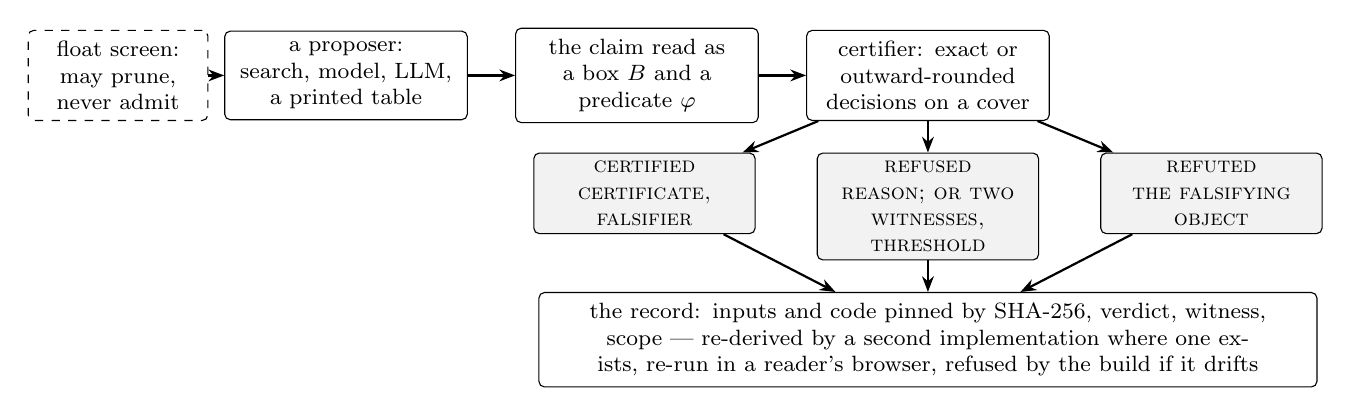
\begin{tikzpicture}[node distance=4mm and 6mm, every node/.style={font=\footnotesize}, box/.style={draw, rounded corners=2pt, align=center, inner sep=4pt, text width=28mm, minimum height=10mm}, verdict/.style={draw, rounded corners=2pt, align=center, inner sep=3pt, text width=26mm, font=\footnotesize\scshape, fill=black!5}, arr/.style={-{Stealth[length=2mm]}, thick}]
\node[box] (prop) {a proposer:\\search, model, LLM,\\a printed table};
\node[box, right=of prop] (claim) {the claim read as\\a box $B$ and a\\predicate $\varphi$};
\node[box, right=of claim] (cert) {certifier: exact or\\outward-rounded\\decisions on a cover};
\draw[arr] (prop) -- (claim); \draw[arr] (claim) -- (cert);
\node[verdict, below=of cert, xshift=-36mm] (c) {certified\\certificate,\\falsifier};
\node[verdict, below=of cert] (f) {refused\\reason; or two\\witnesses, threshold};
\node[verdict, below=of cert, xshift=36mm] (r) {refuted\\the falsifying\\object};
\draw[arr] (cert) -- (c); \draw[arr] (cert) -- (f); \draw[arr] (cert) -- (r);
\node[box, below=of f, text width=96mm] (rec) {the record: inputs and code pinned by SHA-256, verdict, witness, scope --- re-derived by a second implementation where one exists, re-run in a reader's browser, refused by the build if it drifts};
\draw[arr] (c) -- (rec); \draw[arr] (f) -- (rec); \draw[arr] (r) -- (rec);
\node[box, left=of prop, text width=20mm, xshift=4mm, dashed] (screen) {float screen:\\may prune,\\never admit};
\draw[arr, dashed] (screen) -- (prop);
\end{tikzpicture}
\caption{The system. A proposer is never opened and never trusted; its output is read as a claim over a box and decided by a certifier; the verdict, its witness and the pinned inputs form a record that re-runs without the engine.}\label{fig:system}
\end{figure}

\section{The arithmetic}\label{sec:arith}

Proposition~\ref{prop:sound} has one hypothesis, the inclusion property, and the arithmetic exists to secure it. Two kinds are used, and the choice is made per quantity: exact rationals where a tie must be decided or the object is rational, outward-rounded intervals where the quantity is transcendental or the data are long.

\paragraph{Exact rationals.} Numbers are reduced fractions of arbitrary-precision integers. Doubles convert to them losslessly; linear systems are solved by exact elimination, which reports a singular matrix rather than a small pivot; conversion back to a double is for display only. Rational arithmetic decides every sign it is asked, and it is used for the corners of multilinear forms (Section~\ref{sec:multilinear}), the expected counts of a benchmark, polynomial identities, and the ends of enclosures whose comparison must be exact. Decimal literals --- the digits a claimant printed --- are read as the rationals they denote and kept as strings beside their double images, so that a vertex printed to three decimals and an observation printed to four can be found to coincide \cite{P1}.

\paragraph{Outward rounding on doubles.} IEEE-754 arithmetic in round-to-nearest returns, for each of $+, -, \times, \div$, the double nearest the exact result, which therefore lies within half a unit in the last place of the computed one \cite{IEEE754,Goldberg91}. JavaScript cannot set the rounding mode, so directed rounding is emulated: each computed endpoint is moved one unit in the last place outward by stepping its bit pattern.

\begin{proposition}\label{prop:ulp}
Let $\circ \in \{+,-,\times,\div\}$, let $A$, $B$ be intervals of doubles with $0 \notin B$ when $\circ = \div$, and let $\ell$ and $h$ be the round-to-nearest values of the smallest and largest of the endpoint combinations $a \circ b$. If no overflow occurs, then $A \circ B \subseteq [\mathrm{down}(\ell), \mathrm{up}(h)]$, where $\mathrm{down}$ and $\mathrm{up}$ step one double toward $\mp\infty$.
\end{proposition}

\begin{proof}
For these operations the extremes of $a \circ b$ over a product of intervals are attained at endpoint combinations (monotonicity in each argument on each sign region, with $0 \notin B$ for division). The exact extreme lies within half the spacing of the doubles on its side of its round-to-nearest value, and the adjacent double on that side is a whole spacing away (subnormal spacing included), so it lies on the correct side of $\mathrm{down}(\ell)$ and $\mathrm{up}(h)$.
\end{proof}

Division by an interval that contains zero is refused, not extended; a square is clamped at zero; a non-integer power is refused. The widening costs about one bit per operation and nothing at the accuracy the claims need. Where more precision is required --- a constant to be certified to twelve digits, a Catalan or Li$_2$ value --- a separate arbitrary-precision arithmetic carries a binary mantissa of arbitrary length with true directed rounding (floor and ceiling of the shifted integer), and converts its results to doubles outward with an exact check.

\paragraph{Elementary and special functions.} The certifiers of this paper trust no library function, because the platform's \texttt{Math.exp} and \texttt{Math.log} carry no accuracy guarantee in ECMAScript (one older helper that pads the platform's cosine instead is used by four instruments outside this paper's scope, and is listed among the limits in Section~\ref{sec:limits}). Each function is a truncated series evaluated in interval arithmetic plus an explicit bound on the omitted tail: $\exp$ after reduction $x = k\ln 2 + r$, $|r| < 1$, by twenty-four Taylor terms and the tail $|r|^{25}/25!\,(1 - |r|/26)^{-1}$; $\log$ after $x = m\,2^e$ by the series of $\operatorname{atanh}$ in $v = (m-1)/(m+1) \in [0, 1/3)$, whose one-sided tail is valid because $v \ge 0$; $\sin$ and $\cos$ after reduction by an interval enclosure of $\pi/2$, with the box's enclosure forced to $\pm1$ wherever it may contain an extremum; $\ln 2$ and $\pi$ in exact rationals by $\operatorname{atanh}(1/3)$ and Machin's formula, converted outward. Monotone functions on wide boxes are evaluated at the endpoints. The special functions follow the same pattern: $\Gamma$ by Spouge's formula with its error bound taken ten times over; $\ln\Gamma$, $\psi$ and $\psi'$ by Binet's expansion after shifting the argument above twenty, the first omitted term as the bound; the regularized incomplete gamma function by its series with a geometric tail; Bessel functions by their power series with a certified ratio bound; $\operatorname{erfc}$ by Laplace's continued fraction, whose consecutive convergents bracket the value \cite{Abramowitz64}; and inverses ($\Phi^{-1}$, $P^{-1}$) by bisection that moves an end only on a certified sign. The tails are computed in round-to-nearest and are many orders below the one-ulp widening that absorbs them; that margin, not the tail's own rounding, is what makes them safe, and it is stated where it is used.

\paragraph{Long sums.} A running interval sum rounds outward at each of $n$ additions, so its width grows linearly in $n$; at the $\RBuoyN$ hourly values of one buoy it is a thousand times what the terms carry. Each endpoint stream is instead summed by the compensated Sum2 algorithm and the error bound of \cite{Ogita05} is added outward with a factor of two to spare, which is what makes a likelihood over a hundred thousand data an enclosure narrow enough to rank families by \cite{P1}.

\paragraph{Derivatives.} Gradients and Hessians that a certifier needs come from second-order forward differentiation over the same interval arithmetic (a value, a gradient and a Hessian carried through every operation), or from univariate Taylor jets, so that the derivative a proof uses is an extension of the function the proof is about. The remaining families carry hand-written scores and Hessians, evaluated in the same interval arithmetic.

\section{The certifiers}\label{sec:certifiers}

Each certifier below turns a question that is analytic in form into finitely many decisions of the kind Proposition~\ref{prop:sound} covers. None is new; the assembly is, together with the rule that each refuses rather than guesses.

\subsection{A zero, exactly one}
\begin{theorem}[Krawczyk {\cite{Krawczyk69,Neumaier90,Rump10}}]\label{thm:krawczyk}
Let $f : D \subseteq \R^n \to \R^n$ be continuously differentiable, $X \subseteq D$ a box, $\hat x \in X$, $Y$ a nonsingular matrix and $F'(X)$ an interval extension of the Jacobian over $X$. If
\[ K(X) = \hat x - Y f(\hat x) + \bigl(I - Y F'(X)\bigr)(X - \hat x) \subseteq \operatorname{int} X, \]
then $f$ has exactly one zero in $X$.
\end{theorem}
The certifier takes $\hat x$ from a floating-point search, $Y$ as an approximate inverse of the Jacobian at $\hat x$, evaluates $K(X)$ with every datum enclosed by its neighbouring doubles, and inflates $X$ for a bounded number of rounds; if the inclusion never holds the zero is \vF\ with the reason ``no contraction''. A sibling certifier for fixed points in weighted sequence spaces uses the radii-polynomial form of the same argument and requires the contraction factor to be proved below one before it states uniqueness.

\subsection{A maximum in a box}
\begin{proposition}\label{prop:max}
Let $\ell$ be twice continuously differentiable on a convex box $X$, let $\nabla\ell$ have exactly one zero $\theta^\ast$ in $X$, and let the Hessian of $\ell$ be negative definite at every point of $X$. Then $\theta^\ast$ is the unique maximiser of $\ell$ on $X$.
\end{proposition}
\begin{proof}
A function whose Hessian is negative definite on a convex set is strictly concave there, and a critical point of a strictly concave function is its unique maximiser on the set.
\end{proof}
Negative definiteness over the box is proved one of two ways: by Sylvester's criterion on the interval Hessian, its leading principal minors enclosed and proved of alternating sign over all of $X$ (for up to three parameters, with the two enclosures of each symmetric entry intersected); or, where the box's minors are too wide, at the candidate point together with a proof that every Hessian over $X$ is nonsingular --- $|I - A H(X)|\,u < u$ componentwise for a positive vector $u$ and an approximate inverse $A$ --- so that, $X$ being connected and the eigenvalues continuous, no Hessian over $X$ can change its inertia. This is how a maximum-likelihood fit becomes a certificate \cite{P1}. The statement is local: that no better maximum exists elsewhere in the family remains the search's claim, and every fit is stated with that scope.

\subsection{A supremum at a limit}
Some families have no interior maximum on some data: the likelihood rises toward a limit member, and an optimiser prints the last iterate as the fit.
\begin{proposition}\label{prop:limit}
Let $\ell(\mu, \sigma, Q)$ be continuous on $B \times [0, q_1]$ and differentiable in $Q$ on $B \times (0, q_1]$, and let $\partial\ell/\partial Q < 0$ there. Then for every $(\mu, \sigma) \in B$ and every $Q \in (0, q_1]$, $\ell(\mu, \sigma, Q) < \ell(\mu, \sigma, 0)$.
\end{proposition}
The proof is the mean value theorem. With $Q = 1/\sqrt\alpha$ the generalized gamma reaches the lognormal at $Q = 0$ \cite{Prentice74}, and in these coordinates $Q = 0$ is an ordinary point; a proof that the $Q$-score is negative over a neighbourhood of the lognormal fit refuses the family at its edge \emph{with the proof} that every member there is less likely than its limit. A threshold on $\alpha$ in place of this proof hands a different family the verdict at \ANaiveDiff{} of \ABlocks{} cell-blocks of the extreme-value atlas \cite{P1}, which is the cost of a threshold measured.

\subsection{A statement for every input in a box}\label{sec:multilinear}
Three reductions decide a universal statement over a box.

\emph{Bisection with a proposer.} The box is split until each piece's enclosure decides, a floating-point heuristic choosing the coordinate to split and never a verdict; a depth budget bounds the work, and an exhausted budget is an unresolved refusal. To publish a split refusal, the corners are evaluated as thin boxes and one proved witness is kept on each side.

\emph{Monotone implicit functions.} Where a model quantity is the root of an equation monotone in its parameters, the root's range over the box is bracketed by the roots at two corners, and each end counts only when the equation's sign just beyond it is proved. Colebrook's friction law is handled this way: with $x = 1/\sqrt f$ the root of $h(x) = x + (2/\ln 10)\ln(a + bx)$, increasing in $x$, $a$ and $b$, every root over the box lies in $[x^\ast(a_+, b_+), x^\ast(a_-, b_-)]$, and a floating-point Newton iteration only locates the ends \cite{P2}.

\emph{Multilinear forms.}
\begin{lemma}\label{lem:multilinear}
Let $f$ be multilinear on a box $X \subset \R^n$ (affine in each variable when the others are fixed). Then $f(X) = [\min_v f(v), \max_v f(v)]$, the minimum and maximum taken over the $2^n$ vertices of $X$.
\end{lemma}
\begin{proof}
Fix all variables but one; $f$ is affine in it, so its extremes over that side are at the side's ends. Induct over the variables to reach a vertex for each extreme. $f$ is continuous and $X$ connected, so every value between is attained.
\end{proof}
An emissions-abatement estimate, a sum of products of premises each declared as an interval, is such a form. The kernel checks multilinearity syntactically --- every term a monomial in distinct variables, or the corner rule refuses to apply --- and evaluates the $2^n$ corners in exact rationals; the enclosure is then the exact range, not an outer bound, and the two corners at its ends are the witnesses of a split refusal.

\subsection{A sign, exactly}
Geometric predicates --- which side of an edge a point lies on --- are signs of small determinants. Each is evaluated first in double precision and trusted only when its magnitude clears a forward-error bound proved for the inputs \cite{Higham02,Fortune96}: with coordinates bounded by $M$ and $u = 2^{-53}$, the computed $2\times2$ orientation determinant is within $48uM^2$ of the exact one. Below the bound, the sign is recomputed exactly in integers, each decimal literal scaled to a fixed sixty-four places; a literal that would need more is refused rather than rounded. A point on an edge is reported \textsc{on}, an answer a floating-point test does not have. This is the static filter of exact geometric computation \cite{Shewchuk97,Yap97}, written against the literals a file contains rather than against their doubles. Over a contour benchmark it decided \EPredicatesSci{} predicates, \EExactPredicates{} of them in integers \cite{P1}.

\subsection{A polynomial, nonnegative}
A claim $p \ge \gamma$ is certified by an identity $p - \gamma = \sum_i c_i q_i^2$ with rational polynomials $q_i$ and rational weights $c_i \ge 0$, checked by exact coefficient comparison; a negative weight or a nonzero residual refuses, and the residual is printed. Finding the decomposition is a semidefinite program \cite{Parrilo03,PeyrlParrilo08} that stays outside the trust path: the solver proposes, the identity decides. A separate refuter evaluates $p$ at an exact witness point and refutes the claim if $p(w) < \gamma$.

\subsection{A minimum of a cosine polynomial}
The minimum over $x$ of $\sum_{a \in A} \cos(ax)$ is the minimum over $y \in [-1, 1]$ of $P_A(y) = \sum_a T_a(y)$, a polynomial with integer Chebyshev coefficients. The certifier isolates the critical points with a Sturm chain of the square-free part of $P_A'$ on a slightly enlarged interval, refines each by interval Newton in rationals with outward balls around exact Horner values, encloses $P_A$ on each critical interval with the bound $a^2(a^2-1)/3$ of V.~Markov on the second derivative, adds the endpoints $\pm1$ exactly, and returns the hull of the smallest enclosures. A stronger certificate identifies the minimum as an algebraic number --- a resultant, a Sturm count of one inside the enclosure, irreducibility modulo a prime --- and is \vC\ only when all of these hold.

\subsection{Proposers}
Every certifier above takes its candidate from a floating-point search --- Nelder--Mead and Levenberg--Marquardt for a likelihood, Newton for a root, sampling for a minimum, a semidefinite solver for a decomposition, a language model for a construction --- and none of these is ever in the trust path. A proposer may be wrong, slow or adversarial; it can cost a refusal, never a false verdict. The same rule governs forecasts in the system's applications: a forecaster enters as a proposer of boxes, is graded against what is later observed, and stops being admitted when it misses its declared coverage.

\section{The verification discipline}\label{sec:discipline}

Proposition~\ref{prop:sound} makes the verdicts as sound as the code that computes the extensions. The discipline is how the system guards that code. Its rules are stated as engineering because each is a line of code that refuses --- a battery that exits non-zero, a page builder that will not write its page, a numbers generator that will not write a paper's macros --- and this section says where each refusal sits.

\paragraph{Screens prune, never admit.} Floating point decides only what is worth certifying. Every family of the generation loop declares a cheap screen that may only discard candidates and a certifier that is the only authority; the loop can skip on a screen and can record a hit only from the certifier. A screen is itself a claim that it drops nothing it should keep, so the campaign runner plants known answers that must pass every stage and certify before a run may start, refuses a run whose filters lose one, and requires a deliberately simple baseline beside every campaign so that a clever proposer is measured against something \cite{MethodsNote}.

\paragraph{Red controls must fire.} A check that has never gone red is decoration. A red control is a deliberately wrong variant of a test that must be rejected, and a battery whose red controls do not all fire fails, whatever its other checks say. Examples: a determinant whose double-precision value is $+3.6\times10^{-15}$ and whose exact sign is negative, which the filter must send to exact arithmetic; a ``gate'' that evaluates the floating-point model at the centre of the box, which is what a point pipeline does and which the corners must catch; a missing inner certificate, which must refuse a theorem; a bar on the wrong side of an endpoint, which must be refused by name. The test target runs \MtBatteries{} batteries, \MtBatteriesNode{} in JavaScript and \MtBatteriesPy{} in Python, and a wiring check refuses a tree in which that target and the control build's list differ. In the six-lane audit of machine-written manuscripts, \AiMutations{} mutation controls stand beside \AiChecks{} named checks, and the campaign runner ships \CheatsN{} ways to cheat its own reward signal, each caught by a named control \cite{Register}. The methods note records \BugsN{} defects the project shipped and then found: none was found by reading code; each was caught by an impossible number, a calibration, a control, a byte pin or an outside read \cite{MethodsNote}.

\paragraph{Pin the bytes.} Every claim is decided against a held byte sequence named by path and SHA-256 and re-hashed at decision time: the claimant's file, the dataset, the printed table transcribed digit for digit, and the certifying modules themselves, whose digests a ledger records and whose workers refuse other bytes. A page that reports a record refuses to build when a pinned input has changed, when the record was written by a different version of its verifier, or when its battery does not pass; an application build that regenerates a record and finds it different from the committed one refuses and leaves the committed record in place. Files lifted from the laboratory this system grew out of come through a manifest of their source paths and digests.

\paragraph{Independence from the claimant.} The claimant's program is never in the trust path: the decision is re-derived from the published statement and the published bytes, and where a claimant's script was read to settle which identity a manuscript meant, the record says so and the script was not executed. An unqualified ``no shared code'' would not survive a check, because two of the system's own instruments reuse its own code across a producer--checker line; the precise form adopted is that the system \emph{shares no code with the claimant}, and every certificate re-runs with no engine present \cite{Positioning}.

\paragraph{Second implementations.} Where a verdict is the product, a second program written from the specification, in another language and arithmetic and sharing no code, re-derives it (Table~\ref{tab:second}). Not every certifier has one; Section~\ref{sec:limits} names those that do not.

\begin{table}[t]\centering\small
\begin{tabular}{@{}L{0.2\linewidth}L{0.36\linewidth}L{0.36\linewidth}@{}}\toprule
decision & the two implementations & recorded agreement \\\midrule
engineering gate & JavaScript intervals; Python \texttt{decimal} at fifty digits & inside the gate's enclosures at \GRefPoints{} inputs, tightest margin \GRefMargin{} bar \\
abatement kernel & JavaScript exact rationals; Python \texttt{fractions} & \MtAbatVersions{} scenario versions character for character, \MtAbatInterior{} interior points \\
wave-window decisions & JavaScript exact rationals; a clean-room Python verifier from the written specification & every published decision of a day re-decided, the build refusing on one disagreement \\
$\delta_3$ certificates & the claimant's Python verifier; a clean-room JavaScript verifier & \MtDeltaCerts{} of \MtDeltaCerts{} certificates verified by both \cite{Delta3} \\
a Hankel-determinant wall & a lifted arbitrary-precision engine; a standard-library cross-check & \MtZetaRows{} rows re-run bit-identical, \MtZetaCross{} of \MtZetaCross{} cross-checks agreeing \\
\bottomrule\end{tabular}
\caption{Decisions re-derived by a second implementation that shares no code with the first. Each agreement is read from the record that holds it.}\label{tab:second}
\end{table}

\paragraph{Records re-run.} A record is not believed because it was written; it is re-derived. Published records re-run in the reader's browser by the bytes that wrote them and are compared with the record --- by digest for a day of wave-window decisions and a cell of the extreme-value atlas, field by field for an engineering receipt and an abatement registry. A rerun kit lists \MtKitCommands{} commands that re-derive the register's records or verify them with the standard library alone; its one recorded execution, on \MtRunDate{}, ran \MtRunCommands{} of them in about \MtRunMinutes{} minutes on a laptop and compared \MtRunRows{} register rows before and after: \MtRunMoved{} moved, \MtRunFailed{} failed. And the system's own results are offered to outside parties to re-certify without its code; \MtOutsideReruns{} such rerun is recorded so far, the $\lambda(4)$ audit of Section~\ref{sec:record}.

\paragraph{Honest counting.} Every row is derived from a record; a claim with no record gets no row. An aggregate audit counts once and names its most frequent defect. A correction the system adds beside a refuted claim is never counted among the audited corpus's rows; a queued row is not a decided row; refusal kinds are never merged into one total; and every number in this paper and its companions is a macro written by a generator that refuses when a record no longer supports the sentence that quotes it \cite{Register}.

\section{The record}\label{sec:record}

The system's evidence is what it has decided, and every number below is a macro written from the certificate that decided it.

\paragraph{Machine-generated mathematics.} The public register holds \RegRows{} published claims from \RegSources{} sources, decided between \RegFirstDate{} and \RegLastDate{}: \VCertified{} certified, \VRefuted{} refuted, \VPartial{} partial, \VMixed{} mixed, \VRepaired{} repaired, \VNeedsData{} needing data the claimant has not published, and \VQueued{} queued and not counted \cite{Register}. Most claims hold: \RegHolds{} of the \RegDecided{} decided rows name nothing wrong. The defects that appear are of the verifier's kind rather than the mathematician's. A constant posted to a problem thread as a bare decimal is a floating-point product, and parts from the certified enclosure at its \CstarPlace{}th decimal place, by a witness that needs one integer inequality over the exact partial product of the primes up to \CstarLimit{}; witnesses hold only within a verifier's tolerance in \KTolerance{} rows; one checker accepts what its own definition excludes. One row keeps as its history a clause present in a paper's theorem and absent from its formal statement: OpenAI's Navier--Stokes certificate read \textsc{partial} at the announced commit \NsCommit{}, built here over \NsJobs{} modules with only the standard axioms, and \vC\ at the next upstream commit \NsHeadCommit{}, which proved the clause \cite{NSAudit}.

\paragraph{The laboratory's own theorems.} The method runs both ways. The value $\delta_3 = 117/2192$ \cite{Delta3} rests on certificates that two programs sharing no code re-decide, under a battery of \NChecks{} checks with \NReds{} red controls. The value of $\lambda(4)$ \cite{Lambda4} decides \LfClosed{} finite sets across \LfFamilies{} families; on \LfOutsideDate{} an outside audit with no shared code \cite{Lambda4Audit} re-derived the argument from the write-up, re-certified every finite case in interval arithmetic and swept the gcd-reduced sets up to \LfOutsideMax{} as a proof-independent control; its \LfFindings{} documentation findings were folded in and no step broke. That audit is recorded as a row like any other.

\paragraph{Engineering numbers.} A recommendation to raise water injection by 4.2\% on a deep-water flowline, plausible to a reader, is \vF\ \cite{P2}: inputs in the declared envelope give wellhead pressures of \GCornerAbove{} and \GCornerBelow{} bar against a limit of \GRulePwh{} bar, each proved at a corner, and the rule is \textsc{proved} at a pump discharge of \GFlipGreen{} bar or less. Of \GFaults{} injected faults of the kinds an industrial verifier must catch, \GFaultsRefuted{} are refuted and \GFaultsRefused{} refused, each with its reason. A Monte Carlo study of the same recommendation finds exceedances in \MPOver{} of \MDraws{} uniform draws with a worst draw of \MMax{} bar against the proved worst corner of \GCornerAbove{} bar --- the sampling found the risk, and the decision states its extent without a prior over the envelope. A second implementation in fifty-digit decimal arithmetic, sharing no code, lies inside the gate's enclosures at \GRefPoints{} inputs.

\paragraph{Metocean statistics.} Over the open-sea cells of a public global hindcast, \ACertified{} of \AFits{} maximum-likelihood fits are certified maxima, and \AGGLimit{} generalized-gamma fits are refused with the proof of Proposition~\ref{prop:limit}; a scientific library's default call is the maximum it reports on none of \SFits{} fits. Of the \EComparisons{} numbers a contour benchmark printed, \EExact{} are the exact count, two are traced to files rewritten after the count, and \ENotSimple{} of its \EContours{} polygons cross themselves \cite{P1}.

\begin{table}[t]\centering\small
\begin{tabular}{@{}L{0.2\linewidth}L{0.36\linewidth}L{0.36\linewidth}@{}}\toprule
domain & what is decided & the check that shares no code \\\midrule
mathematics & \RegRows{} published claims: constants, constructions, bounds, formal statements & the claimant's checker is never run; one theorem of the laboratory re-certified by an outside group \\
engineering & an operating recommendation over a declared envelope; \GFaults{} injected faults & a fifty-digit decimal implementation, inside the enclosures at \GRefPoints{} inputs \\
metocean & \AFits{} likelihood fits; \EComparisons{} printed contour counts & a library's two answers decided as claims; the counts re-derivable in any exact arithmetic \\
\bottomrule\end{tabular}
\caption{The record by domain. Every entry is a row of a public ledger that the build re-derives; the companion papers report each in full \cite{Register,P2,P1}.}\label{tab:record}
\end{table}

\section{Relation to existing practice}\label{sec:related}

\paragraph{Validated numerics and computer-assisted proof.} Interval arithmetic \cite{Moore09}, interval methods for nonlinear systems \cite{Neumaier90}, verification methods in floating point \cite{Rump10,Rump99}, ball arithmetic \cite{Johansson17} and the computer-assisted proofs they made possible \cite{Tucker02,Hales17} are the certifiers' ancestry, and the system uses them as such. What it adds is not a technique but a setting: the computations are aimed at other parties' claims, the outcome is one of three published words with a witness, and a failure to decide is a result.

\paragraph{Formal proof.} A proof assistant checks a proof against a stated theorem \cite{Lean4,Mathlib20}; what it cannot check is whether the statement is the one intended, and a translation that compiles may not be faithful \cite{Bastounis26}. The system complements formal proof in two ways: it decides the finite and numerical claims that formal libraries do not yet reach, and it audits formal claims at the level where they can fail --- the statement read hypothesis by hypothesis, the build reproduced, the axioms asked of the kernel, the proof replayed by an independent kernel \cite{NSAudit}.

\paragraph{Exact geometric computation.} Floating-point filters with exact fallbacks are standard in computational geometry \cite{Fortune96,Shewchuk97,Yap97}; the contribution here is only to apply them where a benchmark's number is decided, and to keep \textsc{on} as an answer.

\paragraph{Verification, validation and uncertainty quantification.} Verification and validation qualify a model; uncertainty quantification gives a dispersion \cite{OberkampfRoy10}. Neither decides whether a given number holds for every input the engineer has declared, which is the question the epistemic reading of Definition~\ref{def:claim} answers; the two are complementary, and the demonstrator sets them side by side \cite{P2}.

\paragraph{Machine discovery.} Systems that propose mathematics --- conjectures from numerical coincidences \cite{Raayoni21}, constructions from program search \cite{RomeraParedes24,Novikov25} --- each come with an evaluator written by the producer. The system sits downstream of all of them as an independent decider, and the register is the measure of what that independence finds.

\section{What is not claimed, and the limits}\label{sec:limits}

\paragraph{Not claimed.} Interval arithmetic, the Krawczyk operator, floating-point filters, sums of squares and Sturm sequences are not claimed; they are cited. The validity of a declared model is not claimed: a \textsc{proved} engineering number holds for the declared model over the declared envelope, not for the sea or the reservoir. Nothing is certified in the regulatory sense; the word is used in the mathematical sense of Definition~\ref{def:verdicts} only. Nothing is a probability.

\paragraph{Locality and incompleteness.} A certified maximum is the maximum in its box; a global statement over a family would need a branch-and-bound over the family's whole parameter space, which the system does not yet run. The system refuses what it cannot decide, and the refusal rate is a property of each campaign, published with it.

\paragraph{Soundness rests on code.} Proposition~\ref{prop:sound} is a theorem about interval extensions; whether a program computes one is a fact about the program. The defences --- second implementations, red controls, pinned bytes, outside re-runs (Section~\ref{sec:discipline}) --- reduce that risk and do not remove it, and they are not uniform: some certifiers have a second implementation that shares no code, and some, among them the point-in-polygon decider, the cosine-minimum certifier and the likelihood certifier, are re-run in the browser by the same bytes, which checks the record and not the code.

\paragraph{What a read of the code for this paper found.} The refusals that hold are per battery, per page, per record and per paper's numbers; the aggregate test target and the control page report rather than gate --- the target finishes successfully whatever its batteries print, and the control page shows a red battery as red and is still written. The verdict words are declared per instrument rather than in one shared module; the closed vocabulary is enforced where verdicts are published, by the register's builder, which stops on any other word. The certificate constructor requires a falsifier to be stated, not executed. One helper encloses the cosine by padding the platform's value rather than by a series, and is used by four instruments outside this paper's scope; one quadrature routine that is rigorous on dyadic cells of $[0,1]$ is called on another interval by one instrument; one branch of the radii-polynomial certifier returns success without the interval check its other branch makes; one battery labels some positive assertions as red controls; and in the engineering demonstrator a \textsc{proved} consistency check means that the claim meets an outer enclosure, and the discharge thresholds are rounded outward to a tenth of a bar in floating point rather than in directed rounding. None of these touches a verdict reported in the companion papers as far as the read went; each is recorded in the repository's debt register with the instrument it affects, and the system's own rule applies to them --- a check that has not been made is not a check.

\section{Conclusions}\label{sec:conclusions}

cert-machine decides the numbers and claims that machines propose with three verdicts, each carrying the object that justifies it, sound under one hypothesis that the arithmetic is built to secure. Its certifiers reduce the questions that arrive --- a zero, a maximum, a statement for every input, a sign, a nonnegative polynomial, a minimum --- to finitely many exact or outward-rounded decisions; its discipline keeps them honest by code that refuses; and its record, \RegRows{} published claims, an engineering procedure and an extreme-value atlas, is public and re-runs. What it offers those who produce such claims is not a second opinion but a different object beside their number: a verdict with its witness, in which a refusal says what would decide it.

\cmrepro{The macros are written by \texttt{tools/paper-numbers/cert-machine-method.js} and by the generators of the companion papers (\texttt{tools/build-paper-numbers.js}, \texttt{tools/paper-numbers/register.js}, \texttt{ec-benchmark.js}, \texttt{delta3.js}) from the ledgers they name; a record that no longer supports a sentence makes the build refuse. Repository: \url{https://github.com/carlostoledo1891/cert-machine}, commit \MtCommit{}.}

\begin{thebibliography}{99}\small
\bibitem{Abramowitz64} M.~Abramowitz, I.~A.~Stegun, \emph{Handbook of Mathematical Functions}, National Bureau of Standards, Applied Mathematics Series 55, 1964.
\bibitem{Bastounis26} A.~Bastounis, F.~Circelli, A.~C.~Hansen, Navier--Stokes lost in translation: why Lean verification of AI autoformalisation does not guarantee correct natural language proofs, arXiv:2610.08144, 2026.
\bibitem{Delta3} C.~Toledo, The twelve-block colouring is optimal: $\delta_3 = 117/2192$ --- a computer-assisted proof, its certificates re-decided by two programs that share no code, draft, 2026; archived at doi:\ArchiveDoi.
\bibitem{Fortune96} S.~Fortune, C.~J.~Van Wyk, Static analysis yields efficient exact integer arithmetic for computational geometry, \emph{ACM Trans. Graphics} 15 (1996) 223--248.
\bibitem{Goldberg91} D.~Goldberg, What every computer scientist should know about floating-point arithmetic, \emph{ACM Computing Surveys} 23 (1991) 5--48.
\bibitem{Hales17} T.~Hales et al., A formal proof of the Kepler conjecture, \emph{Forum Math. Pi} 5 (2017) e2.
\bibitem{Higham02} N.~J.~Higham, \emph{Accuracy and Stability of Numerical Algorithms}, 2nd ed., SIAM, 2002.
\bibitem{IEEE754} IEEE, \emph{IEEE Standard for Floating-Point Arithmetic}, IEEE Std 754-2019.
\bibitem{Johansson17} F.~Johansson, Arb: efficient arbitrary-precision midpoint-radius interval arithmetic, \emph{IEEE Trans. Computers} 66 (2017) 1281--1292.
\bibitem{Krawczyk69} R.~Krawczyk, Newton-Algorithmen zur Bestimmung von Nullstellen mit Fehlerschranken, \emph{Computing} 4 (1969) 187--201.
\bibitem{Lambda4} C.~Toledo, The value of $\lambda(4)$: a machine-derived proof completing Mercer's Section-5 program, \url{https://carlostoledo.co/reports/lambda4.html}, doi:10.5281/zenodo.22225861 (2026).
\bibitem{Lambda4Audit} rainrzk, erdos510-lambda4-audit, \url{\LfOutsideUrl}, posted on \url{https://github.com/teorth/erdosproblems/issues/\LfIssue} (\LfOutsideDate).
\bibitem{Lean4} L.~de Moura, S.~Ullrich, The Lean 4 theorem prover and programming language, in: \emph{CADE-28}, LNCS 12699, Springer, 2021, 625--635.
\bibitem{Mathlib20} The mathlib Community, The Lean mathematical library, in: \emph{CPP 2020}, ACM, 2020, 367--381.
\bibitem{MethodsNote} None by reading code: the methods note, \url{https://carlostoledo.co/reports/methods-note.html}.
\bibitem{Moore09} R.~E.~Moore, R.~B.~Kearfott, M.~J.~Cloud, \emph{Introduction to Interval Analysis}, SIAM, 2009.
\bibitem{Neumaier90} A.~Neumaier, \emph{Interval Methods for Systems of Equations}, Cambridge University Press, 1990.
\bibitem{Novikov25} A.~Novikov et al., AlphaEvolve: a coding agent for scientific and algorithmic discovery, arXiv:2506.13131, 2025.
\bibitem{NSAudit} C.~Toledo, An audit of the 2026 Navier--Stokes finite-time blowup claim: the formal statement read against Clay's wording and Mathlib's definitions, the Lean proof built and its axioms asked of the kernel, draft, 2026; report at \url{https://carlostoledo.co/reports/navier-stokes.html}.
\bibitem{OberkampfRoy10} W.~L.~Oberkampf, C.~J.~Roy, \emph{Verification and Validation in Scientific Computing}, Cambridge University Press, 2010.
\bibitem{Ogita05} T.~Ogita, S.~M.~Rump, S.~Oishi, Accurate sum and dot product, \emph{SIAM J. Sci. Comput.} 26 (2005) 1955--1988.
\bibitem{OpenAINS} OpenAI, NavierStokesAndEuler, \url{https://github.com/openai/NavierStokesAndEuler}, commits \NsCommit{} and \NsHeadCommit{}, 2026.
\bibitem{P1} C.~Toledo, Certified extreme-value analysis of significant wave height: maximum-likelihood fits and return levels over a public global hindcast, and environmental contours decided exactly, draft v0.2, 2026; \url{https://carlostoledo.co/paper/p1-return-levels.pdf}.
\bibitem{P2} C.~Toledo, A decision procedure for machine-proposed engineering numbers: three-valued verdicts over a declared uncertainty envelope, with witnesses and the threshold that decides, draft, 2026; \url{https://carlostoledo.co/paper/p2-decision-procedure.pdf}.
\bibitem{Parrilo03} P.~A.~Parrilo, Semidefinite programming relaxations for semialgebraic problems, \emph{Math. Programming} 96 (2003) 293--320.
\bibitem{PeyrlParrilo08} H.~Peyrl, P.~A.~Parrilo, Computing sum of squares decompositions with rational coefficients, \emph{Theoret. Comput. Sci.} 409 (2008) 269--281.
\bibitem{Positioning} Positioning: the decisions, \texttt{notes/positioning-decisions-2026-09-03.md}, \url{https://github.com/carlostoledo1891/cert-machine}.
\bibitem{Prentice74} R.~L.~Prentice, A log gamma model and its maximum likelihood estimation, \emph{Biometrika} 61 (1974) 539--544.
\bibitem{Raayoni21} G.~Raayoni et al., Generating conjectures on fundamental constants with the Ramanujan Machine, \emph{Nature} 590 (2021) 67--73.
\bibitem{Register} C.~Toledo, Independent exact certification of machine-generated mathematics: the first register, draft, 2026; \url{https://carlostoledo.co/paper/register.pdf}.
\bibitem{RomeraParedes24} B.~Romera-Paredes et al., Mathematical discoveries from program search with large language models, \emph{Nature} 625 (2024) 468--475.
\bibitem{Rump99} S.~M.~Rump, INTLAB --- INTerval LABoratory, in: T.~Csendes (ed.), \emph{Developments in Reliable Computing}, Kluwer, 1999, 77--104.
\bibitem{Rump10} S.~M.~Rump, Verification methods: rigorous results using floating-point arithmetic, \emph{Acta Numerica} 19 (2010) 287--449.
\bibitem{Shewchuk97} J.~R.~Shewchuk, Adaptive precision floating-point arithmetic and fast robust geometric predicates, \emph{Discrete Comput. Geom.} 18 (1997) 305--363.
\bibitem{Tucker02} W.~Tucker, A rigorous ODE solver and Smale's 14th problem, \emph{Found. Comput. Math.} 2 (2002) 53--117.
\bibitem{Yap97} C.~K.~Yap, Towards exact geometric computation, \emph{Comput. Geom.} 7 (1997) 3--23.
\end{thebibliography}

\end{document}
